\chapter{La Factorisation en Matrices Non-négatives}
\label{chap:NMF}

\section*{\centering Résumé}


\noindent{\small \textbf{
Le fonctionnement de la Factorisation en Matrices Non-négatives (NMF) est présenté dans ce chapitre. Cette méthode consiste à approximer le spectrogramme en amplitude d'un signal audio par le produit de deux matrices positives : $\mathbf{W}$, un dictionnaire composé de spectres audio, et $\mathbf{H}$, la matrice d'activation temporelle. Les différents aspects de son fonctionnement sont décrits : familles de divergences, algorithmes de mise à jour des matrices, méthode d'apprentissage du dictionnaire. Une forme de NMF est également proposée : la NMF \textit{initialisée seuillée} où un dictionnaire, appris sur la source d'intérêt, est mis à jour et dont les éléments relatifs à cette source sont ensuite sélectionnés par une technique de seuillage. Enfin, les différentes contraintes, qui peuvent être apposées sur les matrices de la NMF, sont décrites et notamment la contrainte de régularité temporelle et de parcimonie.}}

\vspace{2cm}

La Factorisation en Matrices Non-négatives étant la méthode retenue pour la suite des travaux, ce chapitre en présente son fonctionnement. Les principes généraux sont dans un premier temps détaillés, puis les différentes approches de cette méthode sont explicitées.

\section{Principe de fonctionnement de la Factorisation en Matrice Non-négatives}
La Factorisation en Matrices Non-négatives (abrégé NMF pour \textit{Non-negative Matrix Factorization} en anglais) est une technique d'approximation linéaire visant à décomposer une matrice $\textbf{V}$ non-négative de dimensions $F \times N$ en un produit de deux matrices tel que

\begin{equation}
\textbf{V} \approx \textbf{WH}
\end{equation}

où $\textbf{W}$ et $\textbf{H}$ sont deux matrices, également non-négatives, de dimensions respectives $F \times K$ et $K \times N$, appelées \textit{dictionnaire} et \textit{matrice d'activation}. Le choix du rang de factorisation $K$ est le plus souvent déterminé afin que la relation $F \times K + K \times N << F \times N$ soit respectée. Dans ce cas, la NMF est une méthode d'approximation dite de faible rang car elle permet la réduction de la dimensionalité des données. 

La contrainte de non-négativité permet d'assurer seulement des combinaisons additives, la soustraction d'information n'est pas possible dans le produit $\mathbf{WH}$. Cela assure ainsi que les éléments du dictionnaire appartiennent bien tous au même domaine non-négatif que les données d'observations $\mathbf{V}$, et donc de leur interprétabilité. En cela, la NMF réalise alors une représentation dite \og par partie \fg{} dans laquelle $\mathbf{W}$ est composée de briques élémentaires qui, additionnées, permettent d'approximer l'ensemble de $\mathbf{V}$. Un exemple de NMF est présenté dans la Figure \ref{fig:ex_NMF}. Chaque colonne $n$ de la matrice $\mathbf{V}$ est décrite comme la somme des éléments de $\mathbf{W}$ pondérés par la colonne $n$ de la matrice $\mathbf{H}$ :

\begin{equation}\label{eq:nmf_h}
\mathbf{v} \approx \mathbf{\tilde{v}} =  \mathbf{Wh}
\end{equation}

où les caractères minuscules représentent des vecteurs colonnes et $n$ est une trame temporelle. Les majuscules dénotent des matrices.

\begin{figure}[t]
\centering
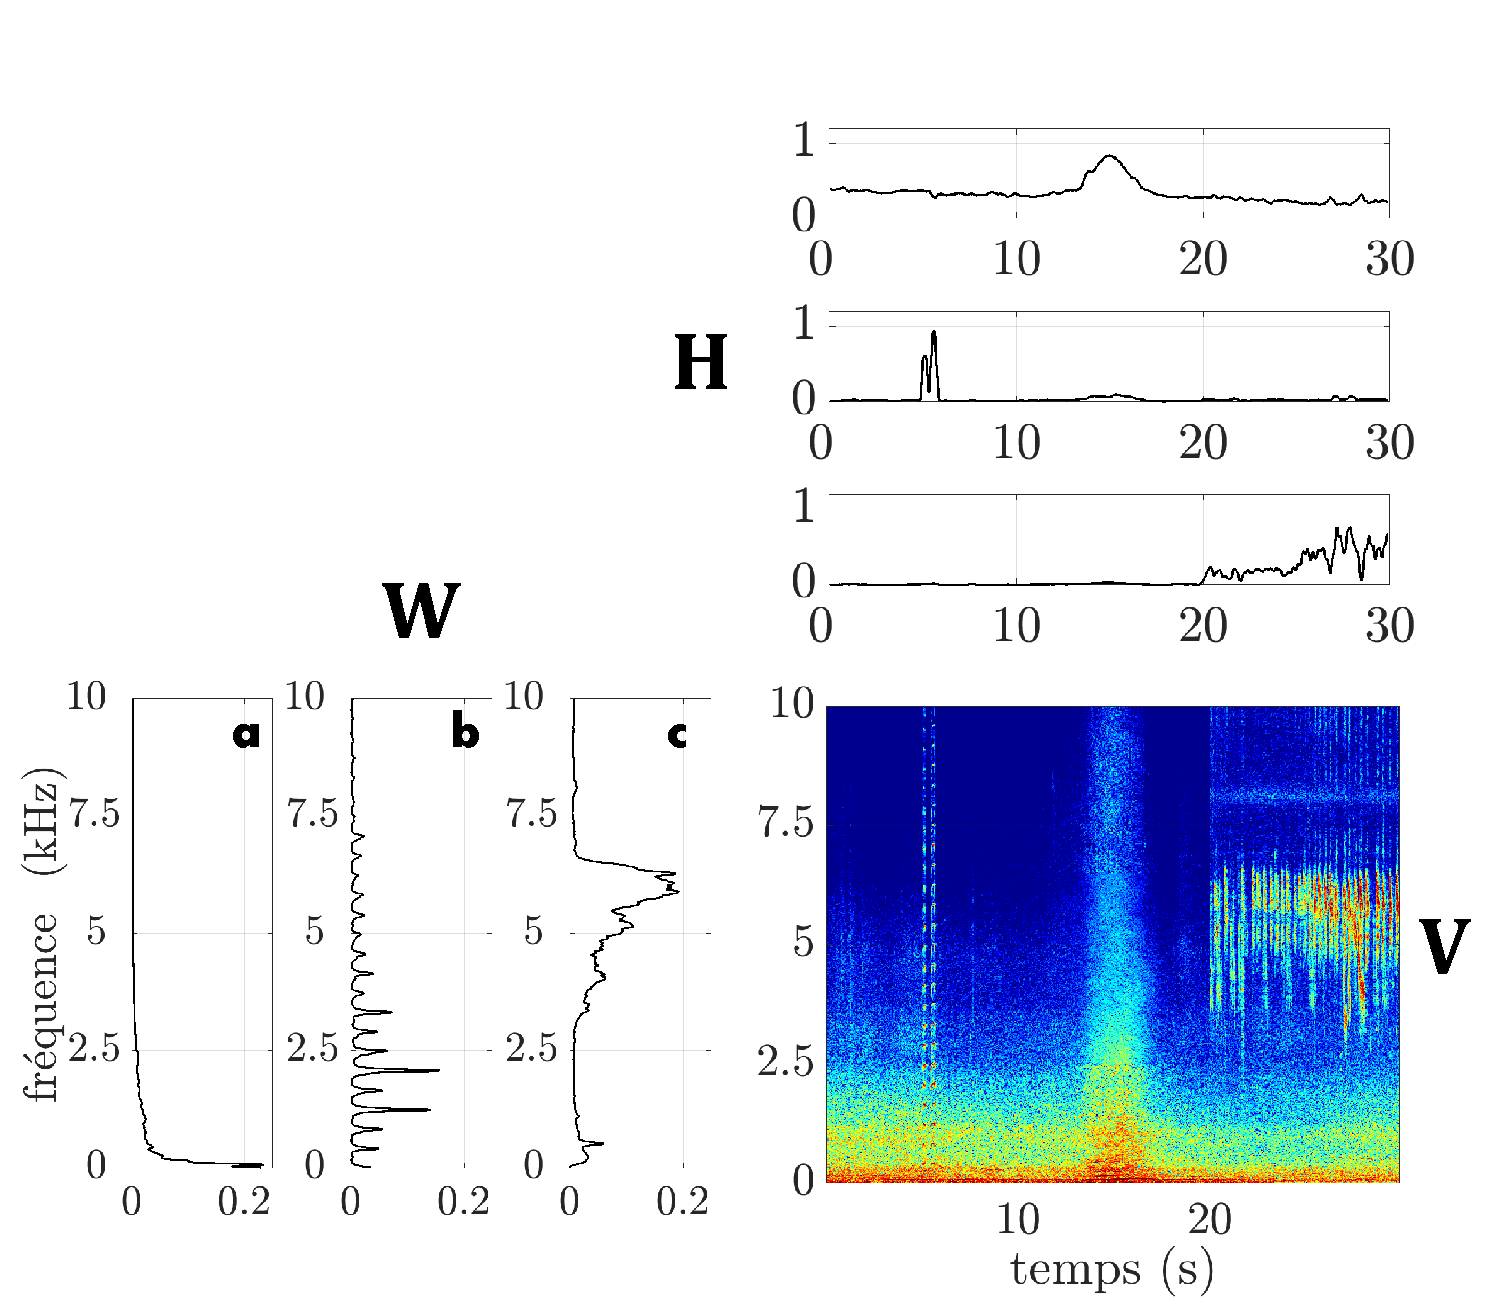
\includegraphics[width=.5\textwidth]{./figures/NMF/schema_introduction_nmf_fr.pdf}
\caption{Exemple d'une NMF pour un signal audio de mixture urbaine composé de 3 sources sonores. $\mathbf{W}$ et $\mathbf{H}$ sont constitués de 3 bases (K = 3) : a) un spectre voiture, b) un spectre de klaxon, c) un spectre d'oiseau.}
\label{fig:ex_NMF}
\end{figure}


Cette méthode est assimilable aux méthodes de factorisation comme l'Analyse en Composantes Principales (ACP), où la contrainte de non-négativité est remplacée par une contrainte d'orthogonalité entre les matrice $\mathbf{W}$ et $\mathbf{H}$, ou l'Analyse en Composantes Indépendantes (ACI) où l'indépendance entre chaque composante est supposée et où il est possible d'obtenir des valeurs négatives. \\

Si la NMF fut introduite pour la première fois par Paatero et Tapper \cite{paatero_positive_1994} en 1994 (mais sous le nom de \textit{Positive Matrix Factorization}), elle doit sa popularité aux travaux de Lee et Seung \cite{lee_learning_1999} dont les résultats furent publiés dans la revue \textit{Nature} en 1999. La NMF a ensuite trouvé de nombreuses applications dans des domaines variés : imagerie \cite{guillamet_introducing_2003, monga_robust_2007}, traitement de texte \cite{xu_document_2003, berry_email_2005}, biologie \cite{gao_improving_2005, chen_constrained_nodate}, gastronomie \cite{hawkins_clustering_2006} ou bien encore pour la recommandation de contenus audio-visuels \cite{luo2014efficient}. Dans le domaine de l'audio, c'est Smaragdis et Brown \cite{smaragdis_non-negative_2003} qui furent les premiers à l'utiliser dans le cas de la transcription d'un morceau de musique polyphonique. Plus généralement, pour un signal audio quelconque, la NMF consiste à approximer son spectrogramme en amplitude ou en puissance, obtenu, par exemple, à partir d'une Transformée de Fourier à Court Terme, à l'aide du dictionnaire $\textbf{W}$ constitué d'un ensemble de spectres sonores dont leurs amplitudes sont pondérées temporellement par les activateurs $\textbf{H}$.

De nombreuses applications de la NMF furent trouvées pour des signaux musicaux et contenant de la parole pour les tâches de détections \cite{dessein2013real}, de reconnaissances de sources \cite{gemmeke2013exemplar}, de classifications \cite{benetos2006musical}, de débruitage \cite{wilson_speech_2008} et de séparations de sources sonores \cite{virtanen_monaural_2007}.

%La NMF pour des signaux environnementaux, c'est-à-dire les signaux qui ne sont ni musicaux ni de parole.
% CITATION avec un peu plus de détaille sur le fonctionnement
%
%\cite{ghoraani2011time} où la NMF est utilisée sur un point d'un long processus
%\cite{gemmeke2013exemplar} pour des sons d'intérieurs
%\cite{mesaros_sound_2015} pour le détection aidé par la NMF
%\cite{satoshi_innami_nmf-based_2012} utilisation de la NMF pour faire de la séparation de sources environnemental.

\section{Fonction de coût et familles de divergences}

Le problème à résoudre lors d'une NMF est celui d'une minimisation où il faut trouver la combinaison optimale de $\mathbf{WH}$ qui sera la plus proche de $\mathbf{V}$. Cela se traduit mathématiquement par la relation \ref{eq:D(V-WH)} :

\begin{equation}\label{eq:D(V-WH)}
\text{min}~D\left(\textbf{V} \Vert \textbf{WH}\right) \quad \text{avec} \quad \mathbf{W} \geq 0, \mathbf{H} \geq 0.
\end{equation}

$D\left(\textbf{V} \vert\vert \textbf{WH}\right)$ est alors une mesure de similarité, appelée \textit{fonction de coût}, qui peut appartenir à différentes familles de divergences comme les divergences de Csiszar \cite{cichocki2006csiszar} et de Bregman \cite{bregman_relaxation_1967, dhillon_generalized_2005}. Cette dernière famille de divergences est la plus couramment utilisée dans le cadre de la NMF. Elle se définit, dans un sous-ensemble convexe $S$ d'un espace de Hilbert, comme :

\begin{equation}\label{eq:Bregdiv}
D_{\Phi}(\textbf{x}\vert\vert \textbf{y}) =
\mathbf{\Phi}(\mathbf{x}) - \mathbf{\Phi}(\mathbf{y}) -
\langle\mathbf{x}-\mathbf{y},\nabla\mathbf{\Phi}(\mathbf{y})\rangle
\end{equation}

où  $\mathbf{x} = (x_1, x_2, \dots x_N)$ et $\mathbf{y} = (y_1, y_2, \dots y_N)$ sont deux distributions, $\mathbf{\Phi}$ est une fonction continue dérivable et strictement convexe défini sur $\mathbb{R}^+$, $\nabla\mathbf{\Phi}(\mathbf{y})$ est le gradient de $\mathbf{\Phi}$ en $\mathbf{y}$ et $\langle .,.\rangle$ est le produit scalaire hermitien. L'équation~(\ref{eq:Bregdiv}) peut être décomposable élément par élément :

\begin{equation}
D_{\Phi}(\mathbf{x}\vert\vert \mathbf{y}) = \sum_{n=1}^N d_{\Phi}(x_n\vert y_n)
\end{equation}

avec $d_{\Phi}(x_n\vert y_n)$, la mesure de similarité entre deux scalaires et $\mathbf{\Phi(x)} = \sum_{n=1}^N \phi(x_n)$. L'équation \ref{eq:Bregdiv} se résume alors à une somme des divergences entre les composantes des distributions $\mathbf{x}$ et $\mathbf{y}$ :

\begin{equation}\label{eq:divBregWise}
D_{\Phi}(\textbf{x}\vert\vert \textbf{y}) = \sum_{n=1}^N \phi(x_n)-\phi(y_n)-\phi'(y_n)(x_n-y_n).
\end{equation}

La fonction de coût s'exprime donc comme la divergence de Bregman appliquée à chaque élément de $\mathbf{V}$ et $\mathbf{WH}$,

\begin{equation}\label{eq:similarite2}
D\left(\textbf{V} \vert\vert \textbf{WH} \right) = \sum_{f = 1}^{F} \sum_{n = 1}^{N} d_{\phi}
\left(\textbf{V}_{fn} \vert \left[ \textbf{WH} \right]_{fn} \right).
\end{equation}


Cette divergence possède plusieurs propriétés :

\begin{enumerate}
\item \textbf{Non-négativité} : $d_{\phi}(x\vert y) \geq 0$.

\item \textbf{Séparabilité} : si $d_{\phi}(x\vert y) = 0$ alors $x = y$.

\item \textbf{Convexité} : $D_{\phi}(\textbf{x}\vert\vert \textbf{y})$ est une fonction réelle strictement convexe pour le 1\ier{} argument mais pas nécessairement pour le second.

\item \textbf{Linéarité} : pour deux fonctions convexes, réelles $\phi_1$ et $\phi_2$,  $d_{\alpha \phi_1 + \beta \phi_2}(x\vert y) = \alpha d_{\phi_1}(x\vert y)+\beta d_{\phi_2}(x\vert y)$ où $\alpha$ et $\beta \in \mathbb{R}^+$.

\item \textbf{Dualité} : pour la fonction convexe conjuguée $\phi^{\ast}$, $d_{\phi^{\ast}}(y^{\ast}\vert x^{\ast}) = d_{\phi}(y \vert x)$.
\end{enumerate}

Si la propriété de non-négativité en fait une famille adaptée pour la NMF, celle de convexité implique qu'il n'est possible que de déterminer un minimum local et donc pas nécessairement la solution exacte au problème énoncé.

\section{Une sous-classe des divergences de Bregman : la $\beta$-divergence}

Dans \cite{banerjee2005clustering}, les auteurs démontrent qu'à chaque divergence de Bregman est associée une famille exponentielle unique $p\left(x\vert \theta,\lambda\right)$:

\begin{align}
 \label{eq:modele_disp_exp}
p\left(x\vert \theta,\lambda\right) &= h(x,\lambda) \exp\left[\lambda^{-1}\left(\theta(y) x-\psi(\theta) \right)\right],\\
 &= g(x,\lambda) \exp\left(-\lambda^{-1} d_{\phi}(x\vert y) \right),  \label{eq:tweedie_breg}
\end{align}

avec $h(x,\theta) $, la fonction de base, $\theta(y)$, le paramètre normal (ou canonique), $\lambda$, celui de la dispersion, $\psi(\theta)$ celui de la normalisation et $g(x,\lambda) = h(x,\lambda)\exp(\lambda^{-1}\phi(x))$. Les paramètres sont reliés entre eux par plusieurs relations $y(\theta) = \frac{d\varphi(\theta)}{d\theta}$, $\theta (y) = \frac{d\phi(y)}{dy}$ et $\frac{d\theta (y)}{dy} = v(y)^{-1}$. Un cas remarquable de distribution est la distribution de Tweedie \cite{jorgensen_exponential_1987} qui relie la variance $v(x)$ à la moyenne (ou espérance) de la distribtion $x$ par une relation polynomiale \cite{yilmaz_alpha/beta_2012} définie par un paramètre de forme $\beta$,

\begin{equation}
v(x) = x^{2-\beta}.
\end{equation}

L'ensemble des divergences de Bregman définies par cette distribution dans l'équation \ref{eq:tweedie_breg} est alors paramétré par le choix de cette valeur $\beta$ et peut être généralisé :

\begin{subequations}\label{eq:divBetaGenerale}
\begin{numcases}{d_{\phi_{\beta}}(x\vert y) =}
    \frac{1}{\beta(\beta-1)}(x^{\beta}+(\beta-1)y^{\beta}-\beta xy^{\beta-1}), & $\beta \in \mathbb{R} \backslash \lbrace 0,1\rbrace$,\label{eq:def_beta}\\
    \dfrac{x}{y}-\log \dfrac{x}{y}-1, & $\beta = 0$,\label{eq:def_divIS}\\
    x\log \dfrac{x}{y} - x + y, & $\beta = 1$.\label{eq:def_divKL}
\end{numcases}
\end{subequations}

Les équations \ref{eq:def_divIS} et \ref{eq:def_divKL} sont des cas limites de l'expression \ref{eq:def_beta}. Chaque paramètre de forme choisi coïncide alors avec une distribution particulière des données : pour $\beta = 1$, la distribution de Tweedie s'apparente à une distribution de Poisson, pour $\beta = 0$, c'est une distribution gamma (ou exponentielle). Dans le cas où $\beta = 2$, cela correspond à la distribution de la loi normale (ou loi de Gauss) de moyenne $\mu$ et de variance $\sigma^2$ :

\begin{align}
p(x \vert \theta, \lambda) & = \frac{1}{\sqrt{2 \pi \sigma^2}}\exp\left(-\frac{1}{2} \left(\frac{x-\mu}{\sigma} \right)^2 \right),\\
& = \frac{1}{\sqrt{2 \pi \sigma^2}}\exp\left(-\frac{1}{\sigma^2}  d_{\phi_{2}}(x\vert \mu) \right)
\end{align}

avec $g(x,\lambda) = \frac{1}{\sqrt{2 \pi \sigma^2}}$, $\lambda = \sigma^2$ et $d_{\phi_{2}}(x\vert \mu)$ qui correspond alors à la distance euclidienne. Ces distances et divergences, déduites de la distribution de Tweedie, sont alors regroupées dans une sous-classe des divergences de Bregman, appelée $\beta$-divergences \cite{hennequin_beta-divergence_2011}. C'est cette famille de divergences qui est la plus couramment utilisée dans le cadre de la NMF. La Figure \ref{fig:allure-divergence} permet d'illustrer le comportement de ces divergences. Dans le cas où $\beta \in \left[ 1,2 \right]$, on constate que $d_{\phi_{\beta}}$ est strictement convexe. En dehors de cet intervalle, les divergences présentent également une partie concave. \\

\begin{figure}[h]
\centering
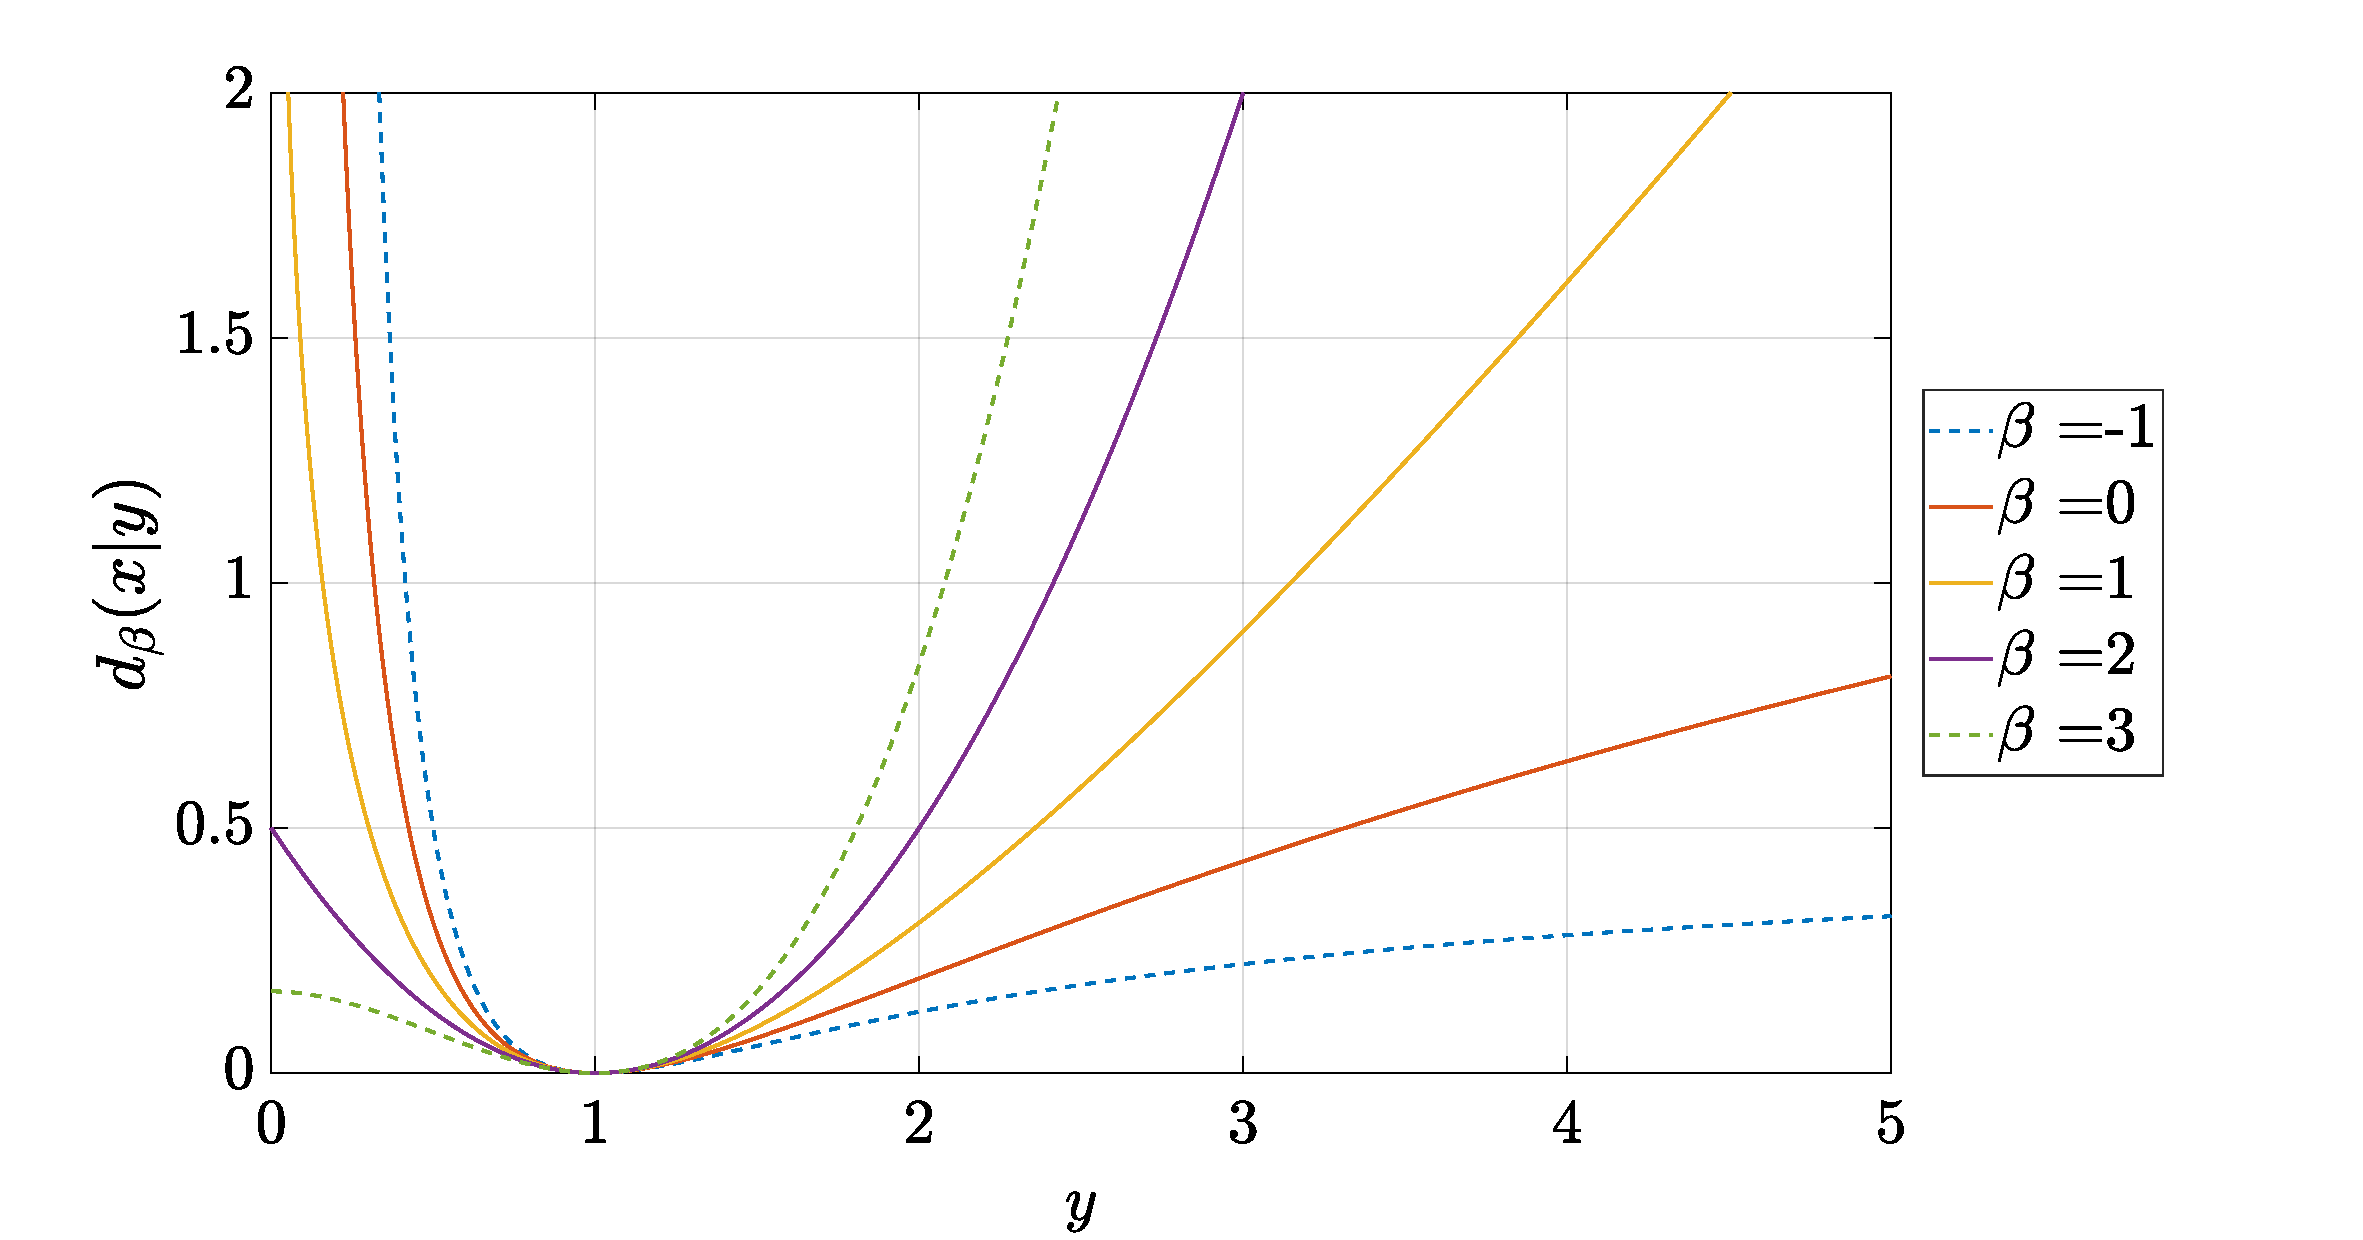
\includegraphics[width=.7\textwidth]{./figures/NMF/betaDiv_exemple.pdf}
\caption{Évolution des $\beta$-divergences pour un cas simple ($x$ = 1).}
\label{fig:allure-divergence}
\end{figure}

Dans le reste du document, par soucis de clarté, les $\beta$-divergences $d_{\phi_{\beta}}$ seront dénommées $d_{\beta}$. Trois $\beta$-divergences associées à des valeurs spécifiques de $\beta  = [0,1,2]$ et à des distributions particulières, sont le plus souvent utilisées dans le cadre de la NMF et sont présentées dans les parties suivantes.

\subsection{Distance euclidienne}\label{part:dist_EUC}
Lorsque $\beta = 2$, la $\beta$-divergence devient \textbf{la distance euclidienne} (abrégé EUC) :

\begin{equation}
d_{{2}}(x\vert y) = \dfrac{1}{2}(x-y)^2.
\end{equation}

Cette métrique équivaut à une mesure de similarité entre les points $x$ et $y$ et se révèle très sensible aux grandes variations entre eux en raison de la présence de la puissance carré. En plus des propriétés des divergences de Bregman, la distance euclidienne en possède 2 autres :
\begin{enumerate}

\item \textbf{Symétrie} : $d_{2}(x \vert y ) = d_{2}(y \vert x)$.

\item \textbf{Inégalité triangulaire} : $d_{2}(x \vert y ) \leq d_{2}(x \vert z ) + d_{2}(x \vert z )$.\\
\end{enumerate}

Comme chaque mesure de distance au point $(x,y)$ possède le même poids que les autres couples de points, il est possible, pour la distance euclidienne, de considérer une pondération $g_{v_{fn}}$  sur les distances selon un critère psycho-acoustique, liée à l'énergie de $v_{fn}$. Cette pondération permet de prendre en compte dans l'erreur de reconstruction, les points temps-fréquences de faibles énergies \cite{virtanen2004separation} :

\begin{equation}
d'_2(v_{fn} \vert w_{fk} h_{kn}) = g_{v_{fn}} d_2 (v_{fn} \vert w_{fk} h_{kn}).
\end{equation}

\subsection{Divergence de Kullback-Leibler}\label{part:div_KL}
L'expression \ref{eq:def_divKL} correspond à \textbf{la divergence de Kullback-Leibler} (abrégé K-L) \cite{kompass_generalized_2007, cichocki_new_2006} . Elle traduit comment une densité de probabilité $\mathbf{x}$ diverge d'une seconde distribution $\mathbf{y}$. En d'autres termes, c'est une mesure de l'information perdue lorsque $\mathbf{y}$ est utilisée pour approximer $\mathbf{x}$. Ne respectant pas les propriétés de symétrie et d'inégalité triangulaire, elle n'est donc pas une distance. La divergence K-L est un cas remarquable puisqu'elle appartient à la fois aux divergences de Bregman et à une autre famille de divergences, les divergences de Csiszar \cite{cichocki_csiszars_2006}.

\subsection{Divergence d'Itakura-Saïto}\label{part:div_IS}
L'expression \ref{eq:def_divIS} est celle de \textbf{la divergence d'Itakura-Saïto} (abrégé I-S) \cite{itakura1968analysis, bertin_les_2009}. Cette divergence est la seule des $\beta$-divergences à posséder la propriété d'\textit{invariance d'échelle} :

\begin{equation}\label{eq:scale_IS}
d_{0}(\lambda x \vert \lambda y) = d_{0}(x \vert y).
\end{equation}

Ce rapport signifie que le même poids est attribué entre les fortes et les faibles valeurs de $\mathbf{x}$. Ainsi, la divergence aux faibles puissances sonores entre $\textbf{V}$ et $\textbf{WH}$ aura la même importance que dans les fortes puissances. La relation \ref{eq:scale_IS} est généralisable à l'ensemble des $\beta$-divergences,

\begin{equation}
d_{\beta}(\lambda x \vert \lambda y) = \lambda^{\beta}d_{\beta}(x \vert y).
\end{equation}


Dans le cas où $\beta > 0$, la divergence est plus influencée par les composantes de fortes amplitudes. À l'inverse, dans le cas où $\beta < 0$, les composantes ayant une faible amplitude ont une plus grande prépondérance. Cette particularité, d'après \cite{fevotte_nonnegative_2009}, est intéressante dans le cadre de signaux audio, et notamment celui des signaux audio musicaux qui possèdent une forte dynamique et dont la puissance décroit exponentiellement en fonction de la fréquence. Une faible valeur de $\beta$ permet alors de mieux prendre en compte les composantes de moindres amplitudes dans la reconstruction du signal.

\subsection{Autres familles de divergences}
Si on s'est attardé à décrire longuement les $\beta$-divergences, d'autres familles de divergences peuvent être utilisées pour la NMF notamment celles appartenant aux divergences de Csiszar (ou appelées $f$-divergences). Cette famille est toutefois moins utilisée que celle de Bregman. Elle se définit comme

\begin{equation}
D_{\Psi} (\mathbf{x} \Vert\mathbf{y}) = \mathbf{x} \mathbf{\Psi} \left( \frac{\mathbf{x}}{\mathbf{y}}\right).
\end{equation}

Elle intègre notamment la distance de variation totale ($\psi(x) = \frac{1}{2}\vert x-1 \vert $), la divergence $\chi^2$ ($\psi(x) = (x-1)^2$), la distance d'Hellinger ($\psi(x) = (\sqrt{x}-1)^2$), les divergences $\alpha$ d'Amari $(\psi(x) = \frac{4}{1-\alpha^2} \left(1-x^{(1+\alpha)/2} \right))$ et la divergence de Kullback-Leibler ($\psi(x) = x\log (x)$). Elle possède plusieurs propriétés (non-négativité, unicité de la solution, symétrie, convexité, dépendance) qui sont détaillées dans \cite{csiszar2004information}.
Enfin, une proposition de généralisation des familles de divergences peut être trouvée dans \cite{cichocki_generalized_2011} où les auteurs généralisent les $\alpha$ et les $\beta$-divergences à travers l'équation  \ref{eq:expression_gen_alpha_beta} :

\begin{equation}\label{eq:expression_gen_alpha_beta}
D_{a, b}(x \vert y) = -\frac{1}{a b}\left(x^{a}y^{\beta}- \frac{a}{a+b}x^{a + b}-\frac{b}{a+b}y^{a+b} \right).
\end{equation}

Les valeurs des coefficients $a$ et $b$ permettent alors d'obtenir soit des $\beta$-divergences ($a = 1$) ou des $\alpha$-divergences ($a+b = 1$) mais également de nouvelles divergences. L'intérêt est d'étendre les familles et les divergences, afin de déterminer de nouveaux algorithmes de mise à jour dont les convergences peuvent être plus rapides, et d'offrir de nombreuses fonctions coûts pouvant mieux s'adapter au problème initial rencontré. Dans le cadre de ce travail, nous nous restreignons aux $\beta$-divergences en raison de leur popularité et des nombreux travaux dans la littérature qui s'y réfèrent.

Notons enfin qu'il n'est pas nécessaire de se restreindre aux divergences bien connues:  \cite{vincent2010adaptive} a, par exemple,  utilisé la NMF dans le cadre de la transcription de signaux musicaux et a déterminé un résultat optimal pour $\beta$ = 0,5. \\

\section{Mise à jour des formes de \textbf{W} et de \textbf{H}}

La minimisation de la $\beta$-divergence entre $\mathbf{V}$ et $\mathbf{WH}$ se résout par un processus d'optimisation qui consiste à faire évoluer la forme des matrices $\mathbf{W}$ et $\mathbf{H}$ itérativement à l'aide d'algorithmes de mise à jour qui dépendent du choix de $\beta$.
Sont présentés ici les algorithmes multiplicatifs les plus couramment utilisés qui garantissent que la contrainte de non-négativité soit respectée.

\subsection{Algorithme heuristique par descente de gradient}

Dans leur premier article consacré à la NMF, Lee et Seung \cite{lee_learning_1999} proposent une première formulation des algorithmes de mises à jour, sans toutefois expliciter leur origine,  pour $\beta  \in \lbrace 1,2 \rbrace$ :

\begin{subequations}\label{eq:WHupdateGD}
\begin{align}
\textbf{W}^{(i+1)} &\leftarrow \textbf{W}^{(i)}\otimes\frac{\left[\left(\textbf{W}^{(i)}\mathbf{H} \right)^{.(\beta-2)}\otimes\textbf{V} \right]\textbf{H}^T}{\left[\textbf{W}^{(i)}\mathbf{H} \right]^{.(\beta-1)}\textbf{H}^T},\\
\textbf{H}^{(i+1)} &\leftarrow \textbf{H}^{(i)}\otimes\frac{\textbf{W}^T \left[\left(\textbf{WH}^{(i)} \right)^{.(\beta-2)}\otimes.\textbf{V} \right]}{\textbf{W}^T \left[\textbf{WH}^{(i)} \right]^{.(\beta-1)}}.
\end{align}
\end{subequations}

Les termes $A\otimes B$ et $\dfrac{A}{B}$ sont des produits de Hadamard (respectivement multiplication et division terme à terme). La minimisation de la fonction \ref{eq:D(V-WH)} se fait alors alternativement en raison de la propriété de convexité de la $\beta$-divergence : pour $\mathbf{W}$ fixé, $\mathbf{H}$ est mis à jour, puis $\mathbf{H}$ est fixé et c'est $\mathbf{W}$ qui est mis à jour.
L'obtention des expressions \ref{eq:WHupdateGD} et la démonstration de leur convergence sont réalisées dans \cite{lee_algorithms_2000} à l'aide de la méthode de descente de gradient. Cette méthode consiste à faire \og glisser \fg {} une solution temporaire le long de la pente négative d'une fonction $f(x)$ afin de converger vers la solution \cite{kivinen_exponentiated_1994} :

\begin{equation}\label{eq:gradient_descent}
x^{(i+1)} \leftarrow x^{(i)} - \eta^{(i)} \nabla f(x^{(i)})
\end{equation}

avec $\eta^{(i)}$ le pas d'apprentissage. Dans le cadre de la NMF, pour la distance EUC, l'équation \ref{eq:gradient_descent} deviennent :

\begin{subequations}\label{eq:WHgradientDescente}
    \begin{align}
     \mathbf{W}^{(i+1)} & \leftarrow \mathbf{W}^{(i)}+\eta_{\mathbf{W}}\left[ \left(\mathbf{V H^T}\right)^{(i)} - \left(\mathbf{W H H^T}\right)^{(i)} \right ], \\
      \mathbf{H}^{(i+1)} & \leftarrow \mathbf{H}^{(i)}+\eta_{\mathbf{H}}\left[ \left(\mathbf{W^TV}\right)^{(i)}-\left(\mathbf{W^T W H} \right)^{(i)}\right ]
    \end{align}
\end{subequations}

avec $\eta_{\mathbf{W}} = \frac{\mathbf{W}}{\mathbf{WHH^T}}$ et $\eta_{\mathbf{H}} = \frac{\mathbf{H}}{\mathbf{W^TWH}}$, les pas d'apprentissages respectifs choisis judicieusement afin d'obtenir les algorithmes de mises à jour \ref{eq:WHupdateGD}. Cette méthode est également développée pour la divergence de Kullback-Leibler dans le même article mais n'est alors pas étendu à l'ensemble de la famille des $\beta$-divergences. La preuve de la convergence des algorithmes est ensuite démontrée à l'aide de l'utilisation d'une fonction auxiliaire (voir partie \ref{part:sub_fonction_aux}).


\subsection{Algorithme multiplicatif par \textit{majorisation-minimisation}}\label{part:majorisation-minimisation}
Une seconde approche \cite{cichocki2006csiszar} consiste à exprimer le gradient de la fonction de coût, $\nabla_x D(x)$, comme la différence entre deux fonctions non-négatives :

\begin{equation}
\nabla_x D(x) = \nabla_x^+ D(x) - \nabla_x^- D(x).
\end{equation}

La fonction de coût $D(x)$ est alors minimisée lorsque, pour un point donné, le gradient est nul ($\nabla_x^+ D(x) = \nabla_x^- D(x)$). Dans le cas de la NMF, les équations de mise à jour de $\mathbf{W}$ et $\mathbf{H}$ deviennent :

\begin{subequations}
    \begin{align}
     \mathbf{W}^{(i+1)} & \leftarrow \mathbf{W}^{(i)}\frac{\nabla_\mathbf{W}^-D(\mathbf{V}\Vert\mathbf{WH})}{\nabla_\mathbf{W}^+D(\mathbf{V}\vert \vert \mathbf{WH})},\\
     \mathbf{H}^{(i+1)} & \leftarrow \mathbf{H}^{(i)}\frac{\nabla_\mathbf{H}^-D(\mathbf{V}\Vert\mathbf{WH})}{\nabla_\mathbf{H}^+D(\mathbf{V}\Vert\mathbf{WH})}.
    \end{align}
\end{subequations}

En considérant des valeurs initiales positives ou nulles dans $\mathbf{W}$ et $\mathbf{H}$, le processus garantit la non-négativité des valeurs itérées. Par cette approche, la minimisation de la fonction de coût de l'équation \ref{eq:D(V-WH)} a, dans un premier temps, été observée sans toutefois être démontrée. Kompass \cite{kompass_generalized_2007} propose une preuve de son efficacité pour $\beta \in \left\lbrace1,2 \right\rbrace$ en considérant une fonction auxiliaire majorante à minimiser. Cette approche est la base de l'algorithme de \textit{majorisation-minimisation} que Févotte et Idier \cite{fevotte_algorithms_2011} ont étendu à l'ensemble des $\beta$-divergences.

\subsubsection{Définition de la fonction auxiliaire}\label{part:sub_fonction_aux}
Pour réaliser une fonction auxiliaire, plusieurs conditions sont à considérer :

\begin{itemize}
\item la mise à jour d'une des deux matrices se fait pour l'autre matrice fixée.
\item Comme l'approximation de la NMF est transposable ($\mathbf{V} \approx \mathbf{WH} \Leftrightarrow \mathbf{V}^T \approx \mathbf{H}^T \mathbf{W}^T$), les mises à jour de $\mathbf{W}$ et de $\mathbf{H}$ sont équivalentes (à cette transposition près).
\item Comme le problème de la minimisation peut se restreindre à chaque composante $n$ (équation \ref{eq:nmf_h}), il est possible de limiter l'étude au cas de la mise à jour de $\mathbf{h}$, un vecteur colonne $n$ issu de $ \mathbf{H}$, pour $\mathbf{W}$ fixé.
\end{itemize}

Considérons le problème suivant :

\begin{equation}\label{eq:costFunctionMM}
\underset{\textbf{h > 0}}{\text{min}}~C(\mathbf{h}) = D(\mathbf{v} \vert\vert \mathbf{Wh})
\end{equation}

avec $\mathbf{W}$ fixé et $\mathbf{v}$ défini à l'équation \ref{eq:nmf_h}. On définit alors la fonction auxiliaire $G(\mathbf{h}\vert \mathbf{h})$ de $C(\mathbf{h})$ telle que :

\begin{subequations}\label{eqs:conditionAux}
\begin{align}
C(\mathbf{h}^{\left(i\right)}) &= G(\mathbf{h}^{(i)}\vert \mathbf{h}^{(i)}) \quad \forall~\mathbf{h} \in \mathbb{R}^+_K,\\
C(\mathbf{h}^{(i)}) &\leq G(\mathbf{h}^{(i)} \vert \mathbf{h}^{(i+1)}) \quad \forall~\mathbf{h} \in \mathbb{R}^+_K.
\end{align}
\end{subequations}

La détermination d'un $\mathbf{h}$ optimal est alors réalisée par un processus itératif afin que

\begin{subequations}\label{eqs:conditionAux2}
\begin{align}
\textbf{h}^{(i+1)} &= \underset{\textbf{h} \geq 0}{\text{arg min}}~ G(\textbf{h}\vert \textbf{h}^{(i)}),\\
C(\mathbf{h}^{(i+1)}) \leq G(\textbf{h}^{(i+1)}\vert\mathbf{h}^{(i)}) &\leq G(\textbf{h}^{(i)}\vert\mathbf{h}^{(i)}) = C(\mathbf{h}^{(i)}).\label{eq:monotonie}
\end{align}
\end{subequations}

La condition \ref{eq:monotonie} permet alors d'obtenir une valeur itérée qui génère un algorithme monotone, c'est-à-dire qu'il certifie la diminution de la fonction de coût à chaque itération. La minimisation de $G(\mathbf{h})$, supposée plus simple, permet,  par extension, celle de $C(\mathbf{h})$. La preuve de la convergence d'un algorithme est présente lorsqu'une suite d'itérations successives tend vers un point $\mathbf{h^*}$ qui satisfait les conditions de Karush-Kuhn-Tucker \cite{fevotte_algorithms_2011, kuhn1982nonlinear}.

\subsubsection{Construction de la fonction auxiliaire}

L'équation \ref{eq:costFunctionMM} peut s'exprimer sous la forme $C(\mathbf{h}) = \sum_f d_{\beta}\left(v_f \vert \left[ \mathbf{Wh} \right]_f \right)$ avec la divergence $d_{\beta}(x \vert y)$ qui se décompose comme une somme d'une fonction convexe,  $\breve{d}(x\vert y)$, concave, $\textit{\textroundcap{d}}(x\vert y)$ et constante, $\bar{d}(x)$ dont les valeurs sont détaillées dans le Tableau \ref{tab:fonctionConcaveConvexe} :

\begin{equation}
d_{\beta}(x\vert y) = \breve{d}(x\vert y) + \textit{\textroundcap{d}}(x\vert y) + \bar{d}(x).
\end{equation}

\begin{table}[t]
\centering
	\begin{tabular}{|*{5}{c|}}
 		\hline
   		 & $\beta < 1$ et $\beta \neq 0$  & $\beta = 0$ & $1 \leq \beta \leq 2$ & $\beta > 2$  \\
   		\hline
   		$\breve{d}(x\vert y)$&$-\frac{1}{\beta -1}xy^{\beta-1}$ & $xy^{-1}$ & $d_{\beta}(x\vert y)$& $\frac{1}{\beta}y^{\beta}$ \\
   		\hline
   		$\breve{d}'(x\vert y)$& $-xy^{\beta-2}$ & $-xy^{-2}$ & $d_{\beta}'(x\vert y)$ & $y^{\beta-1}$\\
   		\hline
   		$\textit{\textroundcap{d}}(x\vert y)$& $\frac{1}{\beta}y^{\beta}$ & $\log y$ & 0 & $\frac{1}{\beta-1}xy^{\beta-1}$ \\
   		\hline
   		$\textit{\textroundcap{d}'}(x\vert y)$& $y^{\beta-1}$ & $y^{-1}$ & 0 & $-xy^{\beta-2}$ \\
   		\hline
   		$\bar{d}(x\vert y)$& $\frac{1}{\beta(\beta-1)}x^{\beta}$ & $x(\log x-1)$ & 0 & $\frac{1}{\beta(\beta-1)}x^{\beta}$\\
   		\hline
 	\end{tabular}
\caption{Fonctions concaves, convexes et constantes selon $\beta$.}
\label{tab:fonctionConcaveConvexe}
\end{table}

Dans le cas où $\beta \in \left\lbrace1,2 \right\rbrace$, la partie concave et constante sont nulles, ce qui se vérifie dans la Figure \ref{fig:allure-divergence}.
La fonction auxiliaire majorante $G(\mathbf{h}^{(i+1)}\vert \mathbf{h}^{(i)})$ est obtenue en majorant ces trois parties séparément : par une inégalité de Jensen pour la partie convexe et par une approximation de Taylor au premier ordre (qui équivaut à sa tangente) pour la partie concave. La fonction auxiliaire $G(\mathbf{h}^{(i+1)}\vert \mathbf{h}^{(i)})$ devient alors 

\begin{multline}\label{eq:fonction_auxiliaire}
G(\mathbf{h}^{(i+1)}\vert \mathbf{h}^{(i)}) = \sum_f \left[ \sum_k \frac{w_{fk}h_k^{(i)}}{\tilde{v}_f} \breve{d}\left(v_f\vert \tilde{v}_f\frac{h_k^{(i+1)}}{h_k^{(i)}} \right) \right]\\
+ \left[ \textit{\textroundcap{d}}'(v_f\vert \tilde{v}_f)
\sum_k w_{fk} (h_k^{(i+1)}-h_k^{(i)})
+ \textit{\textroundcap{d}}(v_f\vert \tilde{v}_f)\right] +\bar{d}(v_f)
\end{multline}

avec $\mathbf{h}^{(i+1)}$, le vecteur $\mathbf{h}$ à mettre à jour, $\mathbf{h}^{(i)}$, le vecteur actuel de $\mathbf{h}$, $\tilde{v}_f= \left[ \mathbf{W h}^{(i)} \right]_f$. La fonction~\ref{eq:fonction_auxiliaire} est alors minimisée en déterminant le zéro de sa dérivée selon $h_k$ :

\begin{equation}\label{eq:derivé-fonc-auxiliaire}
\nabla_{h_k} G(\mathbf{h}^{(i+1)}\vert \mathbf{h}^{(i)}) = \sum_f w_{fk}\left[\breve{d}'\left(v_f\vert \tilde{v}_f\frac{h_k^{(i+1)}}{h^{(i)}_k}\right) + \textit{\textroundcap{d}}'(v_f\vert \tilde{v}_f)\right].
\end{equation}

De l'équation \ref{eq:derivé-fonc-auxiliaire}, l'expression de $h_k^{(i+1)}$ est déterminée :

\begin{align}\label{eq:update_hk}
h_k^{(i+1)} & = h_k^{(i)}\left(\frac{\sum_f w_{fk} v_f \tilde{v}_f^{(\beta-2)}}{\sum_f w_{fk} \tilde{v}_f^{(\beta-1)}}\right)^{\gamma(\beta)},\\
 & = h_k^{(i)}\left(\frac{\nabla_{h_{k}}^- C(\mathbf{\tilde{h}})}{\nabla_{h_{k}}^+ C(\mathbf{\tilde{h}})}\right)^{\gamma(\beta)}
\end{align}

avec

\begin{subequations}\label{eq:gammaGenerale}
\begin{numcases}{\gamma(\beta) =}
    \frac{1}{2-\beta}, & $\beta < 1$, \\
    1, & 1 $\leq \beta \leq 2$,\\
    \frac{1}{\beta-1}, & $\beta > 2$.
\end{numcases}
\end{subequations}

L'algorithme \ref{eq:update_hk} déduit est similaire à l'algorithme heuristique à descente de gradient (équation \ref{eq:WHupdateGD}) et ne diffère que par la présence de l'exposant $\gamma
(\beta)$. Pour $\beta \in \lbrace 1, 2 \rbrace$, où $d_{\beta}(x\vert y)$ est strictement convexe, les deux algorithmes sont même égaux. En dehors de cet intervalle, l'algorithme de \textit{majorisation-minimisation} amène la preuve de la décroissance de l'équation \ref{eq:costFunctionMM} pour tout $\beta$ ce qui n'était qu'observé avec l'algorithme heuristique initial. Ce procédé peut être étendu à $\mathbf{W}$, avec comme fonction auxiliaire $K(\mathbf{w}^{(i+1)}\vert \mathbf{w}^{(i)})$ :

\begin{multline}\label{eq:derivé-fonc-auxiliaireK}
K(\mathbf{w}^{(i+1)}\vert \mathbf{w}^{(i)}) =\sum_f \left[ \sum_k \frac{w_{fk}^{(i+1)}h_{k}}{\tilde{v}_f} \breve{d}\left(v_f\vert \tilde{v}_f \frac{w_{fk}^{(i+1)}}{w_{fk}^{(i)}} \right) \right]\\+ \left[ \textit{\textroundcap{d}}'(v_f\vert \tilde{v}_f) \sum_k (w_{fk}^{(i+1)}-w_{fk}^{(i)}) h_k+ \textit{\textroundcap{d}}(v_f\vert \tilde{v}_f)\right] +\bar{d}(v_f).
\end{multline}

L'expression de $w_{fk}$ est alors déduite :

\begin{equation}\label{eq:update_wfk}
w_{fk}^{(i+1)} \leftarrow w_{fk}^{(i)}\left( \frac{h_k v_f \tilde{v}_f^{(\beta-2)}}{h_k\tilde{v}_{f}^{(\beta-1)}}\right)^{\gamma(\beta)}.
\end{equation}

Les expressions \ref{eq:update_hk} et \ref{eq:update_wfk}, généralisées sous formes matricielles, donnent alors les expressions \ref{eq:WHupdateMM}.

\begin{subequations}\label{eq:WHupdateMM}
\begin{align}
\textbf{W}^{(i+1)} &\leftarrow \textbf{W}^{(i)}\otimes\left(\frac{\left[\left(\textbf{W}^{(i)}\mathbf{H} \right)^{.(\beta-2)}\otimes\textbf{V} \right]\textbf{H}^T}{\left[\textbf{W}^{(i)}\mathbf{H} \right]^{.(\beta-1)}\textbf{H}^T}\right)^{\gamma(\beta)},\label{eq:WupdateMM}\\
\textbf{H}^{(i+1)} &\leftarrow \textbf{H}^{(i)}\otimes\left(\frac{\textbf{W}^T \left[\left(\textbf{WH}^{(i)} \right)^{.(\beta-2)}\otimes\textbf{V} \right]}{\textbf{W}^T \left[\textbf{WH}^{(i)} \right]^{.(\beta-1)}}\right)^{\gamma(\beta)}.\label{eq:HupdateMM}
\end{align}
\end{subequations}


\subsection{Autres approches}

D'autres algorithmes ont été proposés à partir d'approches différentes comme la méthode des moindres carrés alternés \cite{cichocki_regularized_2007, berry_algorithms_2007} qui consiste à minimiser successivement la distance EUC entre $\mathbf{V}$ et $\mathbf{WH}$ en fixant chaque variable alternativement,

\begin{subequations}\label{eq:als}
\begin{align}
\mathbf{W}^{(i+1)} &= \text{arg}~\underset{\mathbf{W} > 0}{\text{min}}~D\left(\mathbf{V} \vert\vert\mathbf{W}^{(i)}\mathbf{H}^{(i)}\right),\\
\mathbf{H}^{(i+1)} &= \text{arg}~\underset{\mathbf{H} > 0}{\text{min}}~D\left(\mathbf{V} \vert\vert\mathbf{W}^{(i+1)}\mathbf{H}^{(i)}\right).
\end{align}
\end{subequations}

Pour résoudre les équations \ref{eq:als}, Zdunek et Cichocki \cite{zdunek2006non} proposent d'utiliser la méthode de Newton alors que Lin \cite{lin_projected_2007} utilise la méthode par projection de gradient. Si ces méthodes offrent des convergences plus rapides que les algorithmes multiplicatifs, elles sont alourdies par la présence de matrice hessienne et ne permettent pas d'intégrer aussi facilement des contraintes sur $\mathbf{W}$ ou $\mathbf{H}$. De plus, ces méthodes de résolutions ne sont adaptées que pour la distance EUC ou la divergence K-L, ce qui restreint les possibilités d'adapter les fonctions coûts aux différents problèmes. En conséquence, bien que plus lent que l'algorithme des Moindres Carrés Alternés, l'utilisation de l'algorithme \textit{majorisation-minimisation} permet l'utilisation de l'ensemble des $\beta$-divergences et d'ajouter plus facilement des contraintes sur les éléments (voir partie \ref{part:NMF_contrainte}).

\section{Analyse Probabiliste en Composantes Latentes}

Il est à noter qu'une autre approche de la NMF existe à travers un pendant probabiliste : l'Analyse Probabiliste en Composantes Latentes (abrégé PLCA pour \textit{Probabilistic Latent Composent Analysis} en anglais) \cite{hofmann_unsupervised_2001, cazau_understanding_2017}. Elle considère l'ensemble des points d'un spectrogramme $V_{F \times N}$ comme le résultat d'un tirage de $F \times N$ variables indépendantes.  Cette distribution suit une loi de distribution discrète paramétrique $P_{\Lambda}\left(f,n\right)$ où $\Lambda$ résume l'ensemble de ces paramètres. En introduisant la variable aléatoire latente (ou cachée) $k$, on obtient :

\begin{align}
P_{\Lambda}\left(f,n\right) &= \sum_k P\left( k \right)P\left(f, n\vert k \right),\\
& = \sum_n P(k)P \left(n \vert k\right)P\left(f \vert k \right)
\end{align}

où $P\left( n \vert k \right)$ est assimilée aux activateurs temporels, $P\left(f \vert k \right)$ aux spectres du dictionnaire (appelés atomes) et $P\left(k \right)$ est le poids relatif de chaque composante. Les paramètres de la loi de distribution $\Lambda$ sont obtenus en maximisant la vraisemblance des observations par un algorithme d'{Esperance-Maximisation} (\textit{Expectation-Maximization} en anglais). Les expressions de mise à jour de chaque distribution sont disponibles en vue de maximiser la vraisemblance (\cite{shashanka_probabilistic_2008}) et permet ainsi de vérifier que la PLCA et la NMF sont des approches similaires d'un problème d'approximation \cite{gaussier_relation_2005}.

Plusieurs variantes de la PLCA existent également comme la PLCA par changement d'invariance (shift-invariant PLCA) \cite{smaragdis_shift-invariant_2007} ou la PLCA par invariance d'échelle (scale-invariant PLCA) \cite{hennequin_scale-invariant_2011} qui permet de transposer des spectrogrammes décomposés en échelle invariante (par une transformation en Q-constant) en une échelle linéaire (obtenue par une TFCT par exemple).

\section{Apprentissage du dictionnaire}

L'utilisation de la NMF nécessite deux étapes : une phase d'apprentissage du dictionnaire et une phase de test (Figure \ref{fig:supervised_learning}) :

\begin{itemize}
\item Durant la phase d'apprentissage, $\mathbf{W}$ et $\mathbf{H}$ sont des matrices dont le contenu est inconnu. Le corpus d'apprentissage est alors soumis à une méthode d'apprentissage permettant de construire le dictionnaire $\mathbf{W}$ (algorithme de clustering \textit{k-means}, NMF\dots). Dans le cas de la NMF, la matrice d'activation obtenue $\mathbf{H_0}$, propre à ce corpus, est alors rejetée, seul $\mathbf{W}$ est conservé pour l'étape suivante. Si on s'arrête à la première étape d'apprentissage, la NMF peut alors être vue comme un algorithme de \textit{clustering} \cite{li2006relationships} et de réduction des données grâce à la contrainte imposée sur les dimensions des matrices ($F \times K + K \times N << F \times N$).
\item Pour la phase de test, le dictionnaire $\mathbf{W}$ obtenu est utilisé sur un corpus de test avec $\mathbf{H}$, une nouvelle matrice d'activation inconnue, qui est à déterminer.
\end{itemize}

\begin{figure}[ht]
\centering
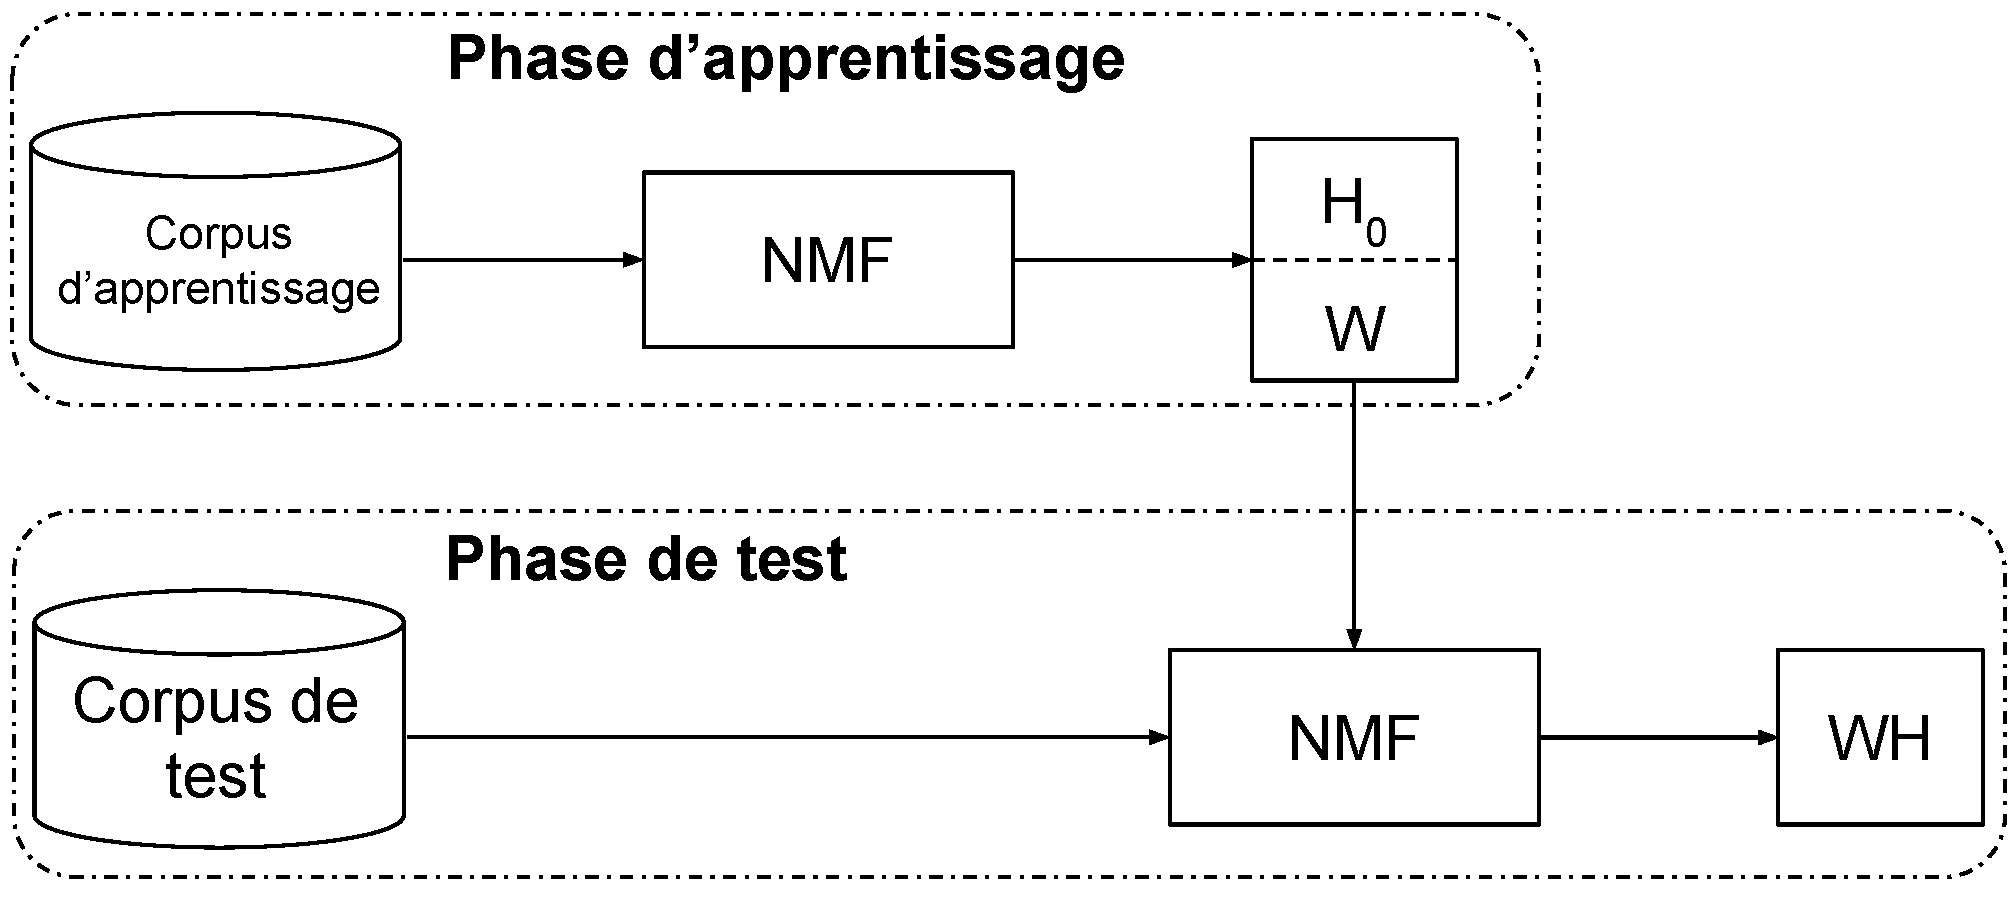
\includegraphics[width=.8\linewidth]{./figures/NMF/NMF_apprentissage.pdf}
\caption{Diagramme en blocs des étapes de la NMF.}
\label{fig:supervised_learning}
\end{figure}

\subsection{Apprentissage supervisé et non-supervisé}
Lorsque les classes de sons du corpus d'apprentissage sont inconnues ou que les échantillons audio sont composés d'un mélange de plusieurs sources, il n'est pas possible de connaitre la classe de son de chaque élément qui constitue $\mathbf{W}$. Toutefois, pour réaliser une séparation de sources, il est nécessaire de classifier les différents éléments entre eux. Une étape de \textit{clustering}, à l'aide d'un algorithme des $k$-NN ($k$ plus proche voisins) par exemple, est alors nécessaire pour classer ces éléments selon un nombre de catégories défini par l'utilisateur. Ce cas correspond à une \textit{NMF non-supervisée}.
À l'inverse, lorsque le jeu de données peut être étiqueté, chaque élément défini dans $\mathbf{W}$ est connu. Ce cas, le plus favorable et le plus simple, correspond à une \textit{NMF supervisée}.
En connaissant la classe des éléments de $\mathbf{W}$, la séparation de sources est réalisable. Pour cela, les éléments relatifs à la source d'intérêt $i$ sont extraits soit directement de $\mathbf{W}$ et de $\mathbf{H}$,

\begin{equation}\label{eq:WH_trafic}
\mathbf{\tilde{V}}_i = \left[\mathbf{WH}\right]_i,
\end{equation}

soit cette séparation est réalisée par un filtre de Wiener (ou masquage doux) :

\begin{equation}
\mathbf{\tilde{V}}_i = \frac{\left[\mathbf{WH}\right]_i}{\mathbf{WH}} \otimes \mathbf{V}.
\end{equation}
\\

\subsection{Apprentissage semi-supervisé}
L'apprentissage du dictionnaire pose la question de la généralisation des connaissances : comment à partir de données limitées obtenir une NMF efficace sur un ensemble de cas divers et variés ?  Cette question se base sur le constat qu'il n'est pas possible de modéliser dans $\mathbf{W}$ l'ensemble des classes de sons qui composent un environnement notamment l'ESU qui est un milieu qui inclut une multitude de sources sonores variables. Pour résoudre ce problème, une des premières solutions est de constituer une base d'apprentissage plus importante que la base de test, en vue d'augmenter la généralisation des connaissances apprises ou leur quantité. Toutefois, cette option n'est parfois pas réalisable soit parce que les données ne sont tout simplement pas disponibles, soit parce que la quantité de données à gérer serait ensuite trop importante et nécessiterait des moyens de calculs puissants pour pouvoir mener à bien l'approximation du signal testé.
Une autre possibilité pour tenter de résoudre cette question est de réaliser un apprentissage semi-supervisé, tel que proposé par \cite{lee_semi-supervised_2010, smaragdis2007supervised} (Figure \ref{fig:semi-supervised_learning}). La NMF semi-supervisée propose de construire un dictionnaire $\mathbf{W}_{F \times (K+J)}$ composé d'éléments appris sur le corpus d'apprentissage, $\mathbf{W_s} $ de dimensions $F \times K$, et d'éléments inconnus, $\mathbf{W_r}$ de dimensions $F \times J$ avec $J << K$. Cette condition est nécessaire afin de focaliser la reconstruction du signal avec les sources présentes dans $\mathbf{W_s}$. L'idée est alors de mettre à jour $\mathbf{W_r}$ lors de la phase de test afin d'y intégrer les autres sources sonores qui ne sont pas apprises dans $\mathbf{W_s}$. On obtient donc

\begin{equation}
\mathbf{V} \approx \mathbf{WH} = \mathbf{W_s} \mathbf{H_s} + \mathbf{W_r} \mathbf{H_r}
\end{equation}


avec $\mathbf{W} = \left[ \mathbf{W_s} \mathbf{W_r} \right]$ et respectivement $\mathbf{H} = \left[ \genfrac{}{}{0pt}{0}{\mathbf{H_s}}{\mathbf{H_r}} \right]$ constituée de la matrice $\mathbf{H_s}_{K \times N}$ et de la matrice $\mathbf{H_r}_{J \times N}$. $\mathbf{H_s}$, $\mathbf{W_r}$ et $\mathbf{H_r}$ sont donc les 3 matrices à déterminer lors de la phase de test à l'aide des algorithmes de mises à jour \ref{eq:WH-SSupdate} \cite{kitamura2014music} : 

\begin{figure}[t]
\centering
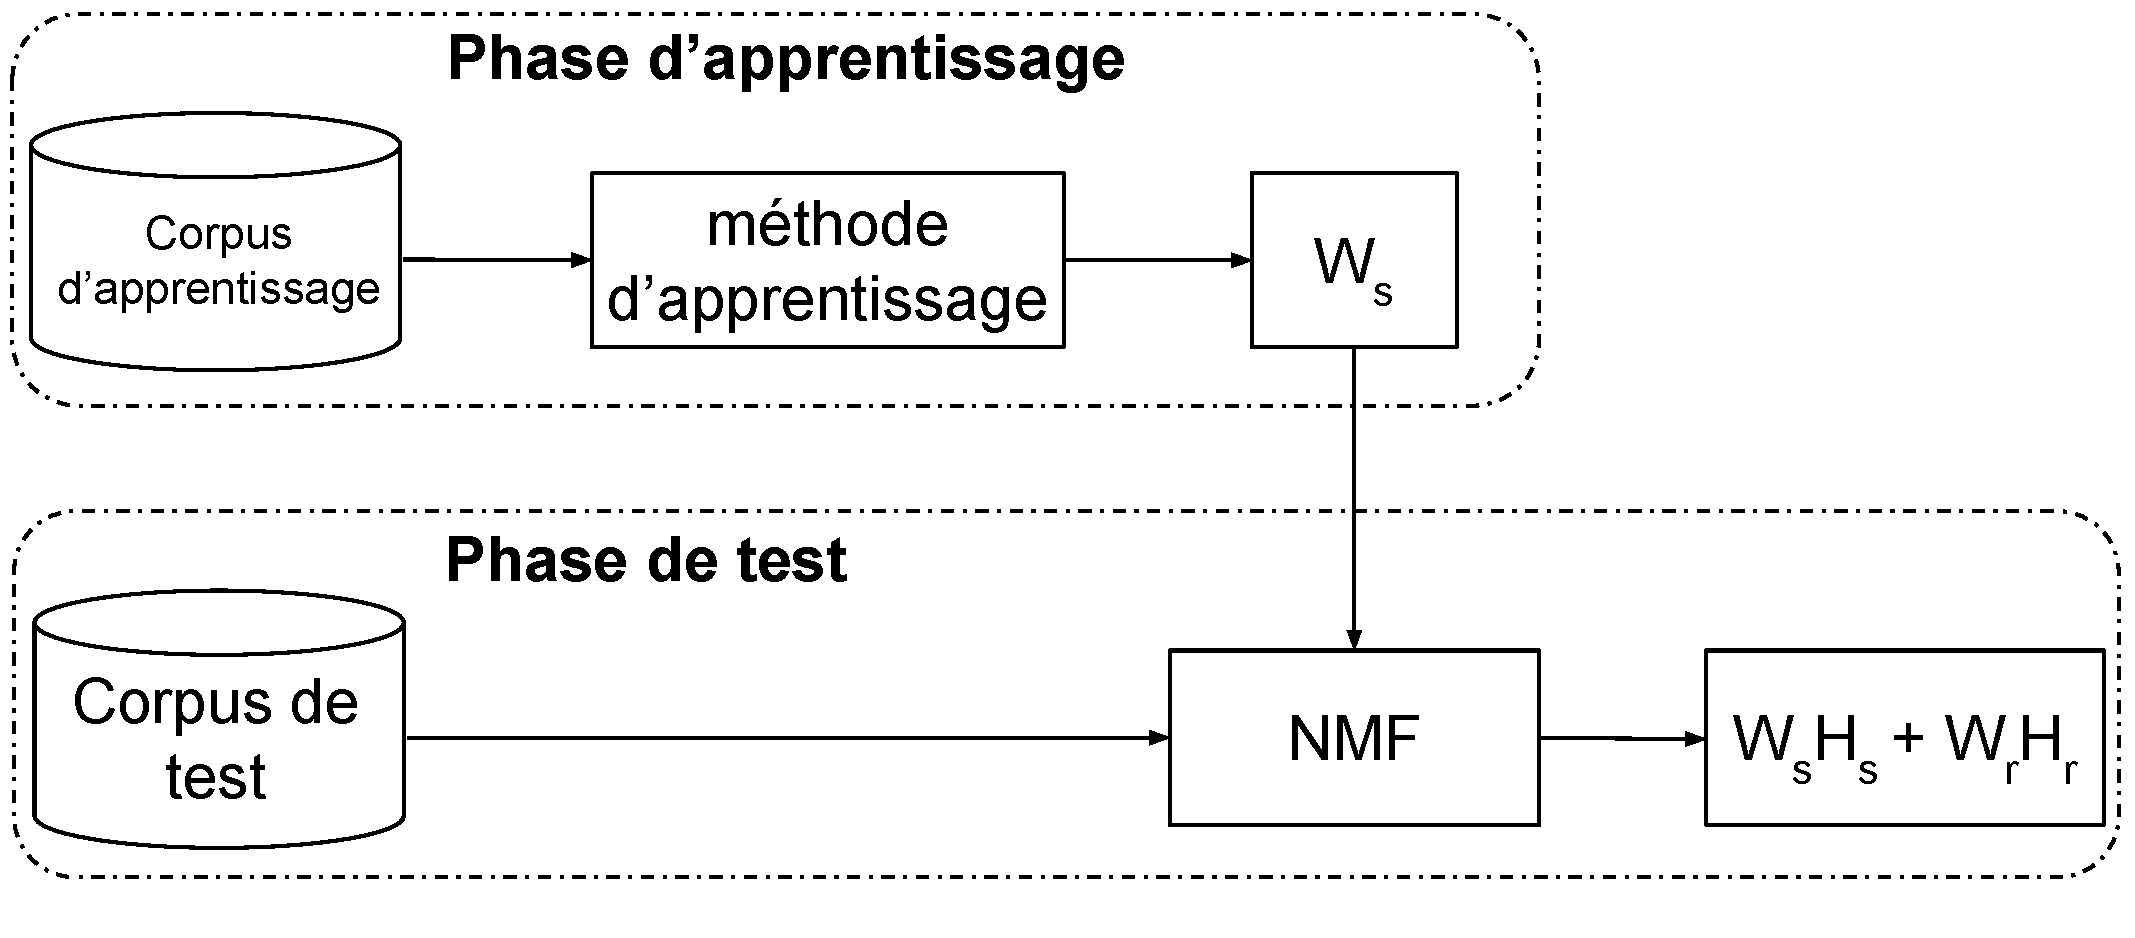
\includegraphics[width=.85\linewidth]{./figures/NMF/NMF_semi-supervised.pdf}
\caption{Diagramme en blocs des étapes de la NMF semi-supervisée.}
\label{fig:semi-supervised_learning}
\end{figure}

\begin{subequations}\label{eq:WH-SSupdate}
\begin{align}
\mathbf{W_r}^{(i+1)} &\leftarrow \mathbf{W_r}^{(i)}\otimes\left(\frac{\left[\left(\mathbf{WH}^{(i)} \right)^{.(\beta-2)}\otimes\mathbf{V} \right]\mathbf{H_r}^T}{\left(\mathbf{WH}^{(i)} \right)^{.(\beta-1)}\mathbf{H_r}^T}\right)^{\gamma(\beta)}\label{eq:W_r_SS}\\
\mathbf{H_r}^{(i+1)} &\leftarrow \mathbf{H_r}^{(i)}\otimes\left(\frac{\mathbf{W_r}^T \left[\left(\mathbf{WH}^{(i)} \right)^{.(\beta-2)}\otimes\mathbf{V} \right]}{\mathbf{W_r}^T \left(\mathbf{WH}^{(i)} \right)^{.(\beta-1)}}\right)^{\gamma(\beta)}\label{eq:H_r_SS}\\
\mathbf{H_s}^{(i+1)} &\leftarrow \mathbf{H_s}^{(i)}\otimes\left(\frac{\mathbf{W_s}^T \left[\left(\mathbf{WH}^{(i)} \right)^{.(\beta-2)}\otimes\mathbf{V} \right]}{\mathbf{W_s}^T \left(\mathbf{WH}^{(i)} \right)^{.(\beta-1)}}\right)^{\gamma(\beta)}.\label{eq:H_s_SS}
\end{align}
\end{subequations}

Dans le cas où $\mathbf{W_s}$ est composé de spectres relatifs au trafic, le produit $\mathbf{W_r} \mathbf{H_r}$ est supposé inclure des éléments qui appartiennent à d'autres classes de sons. L'extraction du signal trafic est réalisée à partir de $\mathbf{W_s}$ et de $\mathbf{H_s}$,

\begin{equation}\label{eq:WSHs_trafic}
\mathbf{\tilde{V}}_{trafic} = \mathbf{W_s H_s}
\end{equation}

Plusieurs applications de cette méthode ont été proposées pour des tâches de séparation de sources dans des signaux musicaux \cite{smaragdis2007supervised} ou pour débruiter des signaux contenant de la voix \cite{mysore2011non, duan2012online}). Dans \cite{lefevre2012semi}, une NMF semi-supervisée est réalisée en contraignant la prépondérance des éléments appris dans la reconstruction du signal afin de faciliter l'annotation pour réaliser de la séparation de sources dans des signaux musicaux.


\section{NMF initialisée seuillée}\label{sec:NMF_TI}

Afin de répondre au problème de généralisation de $\mathbf{W}$, une autre approche est proposée : la \textit{NMF initialisée seuillée} (abrégé NMF IS, à ne pas confondre avec la divergence IS qui est la divergence d'Itakura Saïto). Un dictionnaire initial, $\mathbf{W_0}$, est appris sur la source sonore cible (le trafic routier), puis est mis à jour avec $\mathbf{H}$ lors de la phase de test.
Cette technique permet d'orienter les mises à jour de $\mathbf{W_0}$ vers la source d'intérêt et ainsi de considérer les connaissances obtenues \textit{a priori} sur la source tout en adaptant le dictionnaire à la scène sonore testée. Après $N$ itérations, un dictionnaire $\mathbf{W'}$ est obtenu, unique à chaque scène. Pour estimer le signal \textit{trafic}, chaque élément $k$ du dictionnaire, $\mathbf{W'}$, est comparé à son spectre d'origine dans $\mathbf{W_0}$ afin de déterminer s'il est encore assimilable à un spectre \textit{trafic}. La comparaison des 2 éléments est réalisée à travers le calcul de leur similarité cosinus :

\begin{equation}\label{eq:similarite_cosinus}
 D_{\theta}(\mathbf{W_0}\Vert\mathbf{W'}) = \frac{\mathbf{W_0}.\mathbf{W'}}{\Vert\mathbf{W_0}  \Vert. \Vert\mathbf{W'} \vert \vert}
\end{equation}

qui détermine le cosinus de l'angle $\theta$ formé entre les vecteurs $\mathbf{w_0}$ et $\mathbf{w'}$ par le rapport entre leur produit scalaire et leur norme. Dans la suite du document, on se référera à cette distance sous l'abréviation $D_{\theta}$. Cette métrique est invariante d'échelle et est normée entre -1 et 1 :

\begin{itemize}
\item si $D_{\theta} = 1$, les deux vecteurs sont strictement identiques, $\mathbf{w'}$ est alors considéré comme un élément \textit{trafic},
\item si $D_{\theta} = 0$, les deux vecteurs sont orthogonaux, $\mathbf{w'}$ n'est pas une élément \textit{trafic} et est donc rejeté,
\item si $D_{\theta} = -1$, les deux vecteurs sont opposés. Ce cas n'est toutefois pas possible en raison de la contrainte de non-négativité.\\
\end{itemize}

La similarité entre $\mathbf{W_0}$ et $\mathbf{W'}$ correspond alors à une suite de valeurs comprises entre 0 et 1 puis représentées à travers 2 fonctions (Figure \ref{fig:resume_simil}) :

\begin{itemize}
\item une fonction linéaire, $f_{LIN}(k) = D_{\theta}$,
\item une fonction sigmoïde, $f_{SIG}(k) = \sfrac{1}{\left(1+\exp({-\lambda D_{\theta}}\right)}$ avec $\lambda$ le paramètre d'inflexion de la fonction. Cet opérateur réduit la fenêtre de variation de la distance $D_{\theta}$, en diminuant les valeurs élevées et en augmentant les valeurs proches de 0.\\
\end{itemize}

\begin{figure}
    \centering
    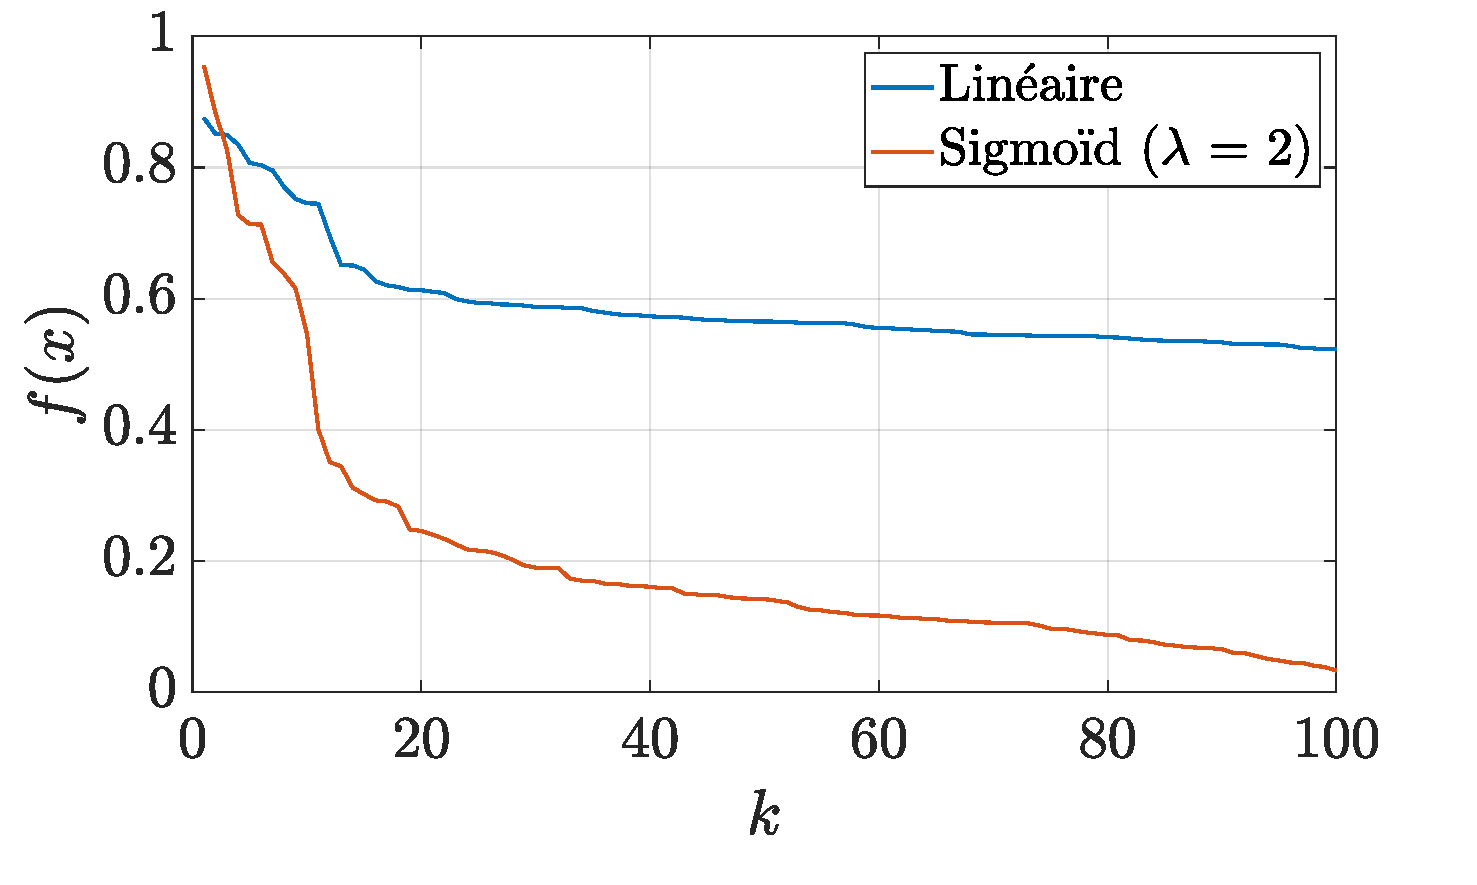
\includegraphics[width=0.7\linewidth]{./figures/NMF/lin_sig.pdf}
    \caption{Similarité cosinus pour une représentation linéaire et sigmoïdienne de la distance $D_{\theta}(\mathbf{W_0} \Vert \mathbf{W'})$ trié dans l'ordre décroissant avec un seuillage dur $t_h$ = 0,6. }
    \label{fig:resume_simil}
\end{figure}

L'extraction du signal \textit{trafic} est réalisée en pondérant alors le produit $\mathbf{W'H}$ tel que

\begin{equation}
\mathbf{\tilde{V}}_{trafic} = \alpha \otimes \left[\mathbf{W'H} \right]
\end{equation}

avec $\alpha = \left[\alpha_1, \alpha_2 \dots \alpha_K \right]$ qui est défini à partir du calcul de similarité (équation \ref{eq:similarite_cosinus}) et d'une méthode de seuillage. 2 méthodes de seuillages sont envisagées :

\begin{itemize}
\item le seuillage dur (\textit{hard thresholding}) \cite{donoho1994threshold} qui consiste à ne considérer dans $\mathbf{W}_{trafic}$ que les éléments de $\mathbf{W'}$ dont la similarité cosinus est supérieure à une valeur seuil $t_h$ :

\begin{subequations}\label{eq:seullageDur_def}
\begin{numcases}{\alpha_k =}
	0 & si \quad $f(k) \leq t_h$,  \\
	1 & si \quad $f(k) > t_h$,
\end{numcases}
\end{subequations}

\item le seuillage \textit{firm} \cite{fornasier2008iterative} qui consiste à pondérer les éléments situés entre deux seuils $t_{f,1}$ et $t_{f,2}$ avec $t_{f,1} < t_{f,2}$, en les normalisant entre 1 et 0 :


\begin{subequations}\label{eq:seuillageFirm_def}
\begin{numcases}{\alpha_k =}
    0, & \text{si}  $f(k) \leq t_{f,1}$, \\
    \Vert f(k)\Vert, & \text{si}  $t_{f,1} < f(k) \leq t_{f,2}$,\\
    1, & \text{si}  $f(k) > t_{f,2}$
\end{numcases}
\end{subequations}
avec $\Vert f(k)\Vert = \frac{f(k)-\min(f(k))}{\max(f(k))-\min(f(k))}$
\end{itemize}

L'allure des pondérations $\alpha$ pour le seuillage dur et \textit{firm} est résumé en Figure \ref{fig:seuillage}.

\begin{figure}
\centering
	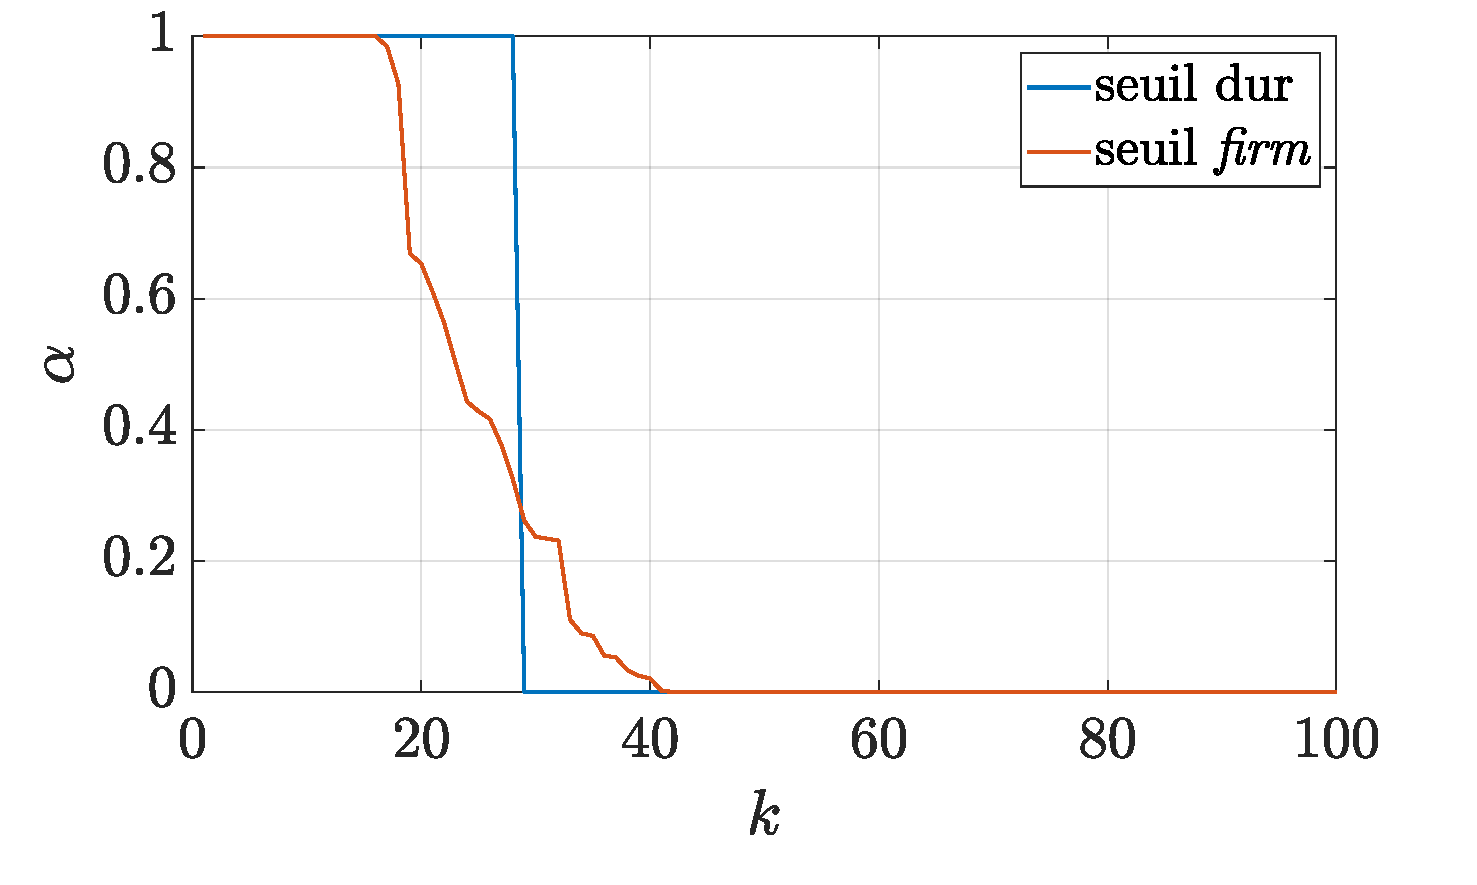
\includegraphics[width=.7\textwidth]{./figures/NMF/seuillage.pdf}
  \caption{Pondération $\alpha$ appliquée à $\mathbf{W'}$, exprimé linéairement, composé de 100 bases avec pour seuil $t_h = 0,2$ (seuillage dur) et $t_{f,1} = 0,15$ et $t_{f,2} = 0,30$ (pour le seuillage \textit{firm}).}
  \label{fig:seuillage}
\end{figure}

On résume les différentes étapes de la NMF IS au travers de l'algorithme \ref{alg:NMF-IS}.

\begin{algorithm}
\caption{NMF initialisée seuillée}
\begin{algorithmic}
\STATE Initialisation de $\mathbf{W_0}$ sur le corpus d'apprentissage
\FOR{i = 1 : nombre itération}
	\STATE mise à jour de $\mathbf{W_0}$
	\STATE mise à jour de $\mathbf{H}$
\ENDFOR
\STATE Calcul de la similarité cosinus $D_{\theta}(\mathbf{W_0} \Vert \mathbf{W'})$
\IF{représentation sigmoïde}
	\STATE $D_{\theta}(\mathbf{W_0} \Vert \mathbf{W'}) = \sfrac{1}{\left(1+\exp({-\lambda D_{\theta}(\mathbf{W_0} \Vert \mathbf{W'})}\right)}$
\ENDIF

\IF{seuillage \textit{dur}}
	\STATE $\alpha$ définit selon Eq. \ref{eq:seullageDur_def}
\ELSIF{seuillage \textit{firm}}
	\STATE $\alpha$ définit selon Eq. \ref{eq:seuillageFirm_def}
\ENDIF
\STATE $\mathbf{\tilde{V}}_{trafic} = \alpha \mathbf{W'H}$
\end{algorithmic}
\label{alg:NMF-IS}
\end{algorithm}

L'intérêt de cette approche est qu'elle permet, par la mise à jour du dictionnaire $\mathbf{W_0}$ de modéliser directement la source sonore \textit{trafic} avec les effets de la propagation de l'environnement sur la propagation sonore. En effet, la NMF supervisée et semi-supervisée possède un dictionnaire fixe (ou dans une grande partie fixe pour la semi-supervisée) avec lequel elles doivent modéliser l'ensemble de cette source. Par rapport au problème posé dans la partie \ref{part:problème}, elles  contiennent dans $\mathbf{W}$, la source $\hat{s}_{v_j}(f)$. La NMF IS en calculant $\mathbf{W'}$ permet une approximation de $M_i$ dont les composantes dans $\mathbf{W'}$ incluent les effets de propagation de l'environnement urbain. L'extraction du signal \textit{trafic} de $W'H$ permet alors de déterminer $\hat{S}_{tr.}(f)$, ce qui permet une plus grande généralisation de la méthode. Toutefois, en mettant à jour la forme de chaque élément, on perd la supervision du dictionnaire. La méthode de seuillage pour déterminer les composante \textit{trafic} génère alors le risque de considérer des éléments de la classe \textit{interférante} si le(s) seuil(s) $t_h$ (ou $t_{f,1,2}$) sont trop faibles ou bien pas assez d'éléments si ils sont trop élevés.

\section{NMF avec contraintes}\label{part:NMF_contrainte}
Les différentes variantes de la NMF présentées ne sont soumises, jusqu'ici, qu'à la contrainte de non-négativité avec pour objectif la minimisation de l'équation \ref{eq:D(V-WH)}. Toutefois, l'ajout de contraintes sur l'apprentissage du dictionnaire ou sur l'allure de la matrice d'activation est possible suivant les connaissances que l'on a \textit{a priori} de ces éléments. Ces contraintes sont alors prises en compte dans la fonction de coût \ref{eq:D(V-WH)} par l'ajout d'un second terme pondéré $C(\mathbf{W},\mathbf{H})$. Le problème devient alors :

\begin{equation}\label{eq:costFunctionPenalized}
\text{min}~D\left(\textbf{V} \Vert \textbf{WH}\right) + \alpha C(\mathbf{W},\mathbf{H}) \quad \text{avec} \quad \mathbf{W} \geq 0, \mathbf{H} \geq 0.
\end{equation}

Si l'allure de $\mathbf{W}$ ou $\mathbf{H}$ n'est pas celle souhaitée, la fonction de coût \ref{eq:costFunctionPenalized} augmente. Les algorithmes de mise à jour vont alors considérer cette contrainte afin de favoriser les matrices qui permettent de minimiser au mieux cette fonction de coût. Le terme de pondération $\alpha$ permet de faire varier le poids de la contrainte : plus ce terme est grand et plus son influence sera prépondérante. Plusieurs types de contraintes sont décrites et serviront dans la suite de l'étude.

\subsection{Contrainte de parcimonie}\label{part:sparsness}
Une des premières contraintes employées est celle de la parcimonie \cite{hoyer_non-negative_2004, le2015sparse} : c'est-à-dire l'utilisation d'un nombre réduit d'éléments du dictionnaire à chaque instant $t$. Cette contrainte renforce la représentation par partie de la NMF en pénalisant les termes qui seraient non nuls. Elle trouve notamment son intérêt dans le cas d'une représentation \textit{sur-complète} du dictionnaire, c'est à dire $K > \max(F,N)$ où l'ajout de la contrainte parcimonieuse permet de réduire la complexité du problème \cite{eggert2004sparse}. Dans un premier temps, Hoyer \cite{hoyer_non-negative_2004} propose une contrainte telle que

\begin{equation}
C(h_k) = \frac{\sqrt{N}-\left( \sum_{n=1}^N \vert h_{kn} \vert \/ \sqrt{\sum_{n = 1}^N h_{kn}^2} \right)}{\sqrt{N}-1}
\end{equation}

qui équivaut au rapport de la norme $\ell_1$ et $\ell_2$ normalisée de $h_{kn}$. Ce rapport est ensuite défini tel que $C(h_k) = C_h$, une valeur constante définie qui fixe la quantité de parcimonie souhaitée dans $\mathbf{H}$. Un algorithme de gradient de descente permet ensuite, sous cette contrainte, de résoudre l'équation \ref{eq:D(V-WH)}. Virtanen \cite{virtanen_monaural_2007} propose l'ajout d'une contrainte $C_{sp}(\mathbf{h})$, le plus souvent considérée comme la norme $\ell_1$ des éléments de $\mathbf{H}$,

\begin{equation}\label{eq:sparsness}
C_{sp}(\mathbf{h}) = \sum_k h_{kn}.
\end{equation}

Cette pénalisation peut facilement être prise en compte dans les algorithmes de \textit{majorisation-minimisation} :

\begin{equation}
\underset{\textbf{h > 0}}{\text{min}}~C(\mathbf{h}) = D(\mathbf{v} \vert\vert \mathbf{Wh}) + \alpha_{sp} C_{sp}(\mathbf{h})
\end{equation}

avec $\alpha_{sp}$, la pondération respective à la contrainte de parcimonie. La fonction auxiliaire pénalisée $G_p(\mathbf{h}^{(i+1)}\vert \mathbf{h}^{(i)})$ devient alors

\begin{equation}
G_p(\mathbf{h}^{(i+1)}\vert \mathbf{h}^{(i)}) = G(\mathbf{h}^{(i+1)}\vert \mathbf{h}^{(i)})+ \alpha_{sp}C_{sp}(\mathbf{h}^{(i+1)})
\end{equation}

et a pour dérivée selon $h_k$

\begin{equation}\label{eq:derivé-fonc-auxiliaireSparse}
\nabla_{h_k} G_p(\mathbf{h}^{(i+1)}\vert \mathbf{h}^{(i)}) = \sum_f w_{fk}\left[\breve{d}'\left(v_f\vert v_f^{(i)}\frac{h_k^{(i+1)}}{h_k^{(i)}}\right) + \textit{\textroundcap{d}}'(v_f\vert v_f^{(i)})\right]+\alpha_{sp}.
\end{equation}

L'algorithme de mise à jour de $\mathbf{H}$ devient alors

\begin{subequations}\label{eq:h_sparsity}
\begin{numcases}{\textbf{H}^{(i+1)} \leftarrow}
  \textbf{H}^{(i)} \otimes\left(\frac{\textbf{W}^T \left[\left(\textbf{WH}^{(i)} \right)^{(\beta-2)} \otimes \textbf{V} \right]}{\textbf{W}^T \left[\textbf{WH}^{(i)} \right]^{(\beta-1)}+ \alpha_{sp}}\right)^{\gamma(\beta)} & $\beta < 2$,\label{eq:h_sparsity_1}\\
    \textbf{H}^{(i)} \otimes\left(\frac{\textbf{W}^T \left[\left(\textbf{WH}^{(i)} \right)^{(\beta-2)} \otimes \textbf{V} \right]-\alpha_{sp}}{\textbf{W}^T \left[\textbf{WH}^{(i)} \right]^{(\beta-1)}}\right)^{\gamma(\beta)}, & $\beta \geq 2$.\label{eq:h_sparsity_2}
\end{numcases}
\end{subequations}

Dans le cas où $\beta \geq 2$, la contrainte apparait au numérateur et est soustractive. Ce comportement peut être problématique dans le cadre de la non-négativité suivant la value de $\alpha_{sp}$ \cite{fevotte_algorithms_2011}. En Figure \ref{fig:sparsity_example}, un exemple de l'effet de la parcimonie sur l'allure d'un élément $j$ de la matrice $\mathbf{H}$ pour 3 valeurs de parcimonie. Avec l'augmentation de la valeur de la pondération, certaines activations présentes lorsque la contrainte est absente, mais de faibles amplitudes, deviennent nulles. 

\begin{figure}[h]
\centering
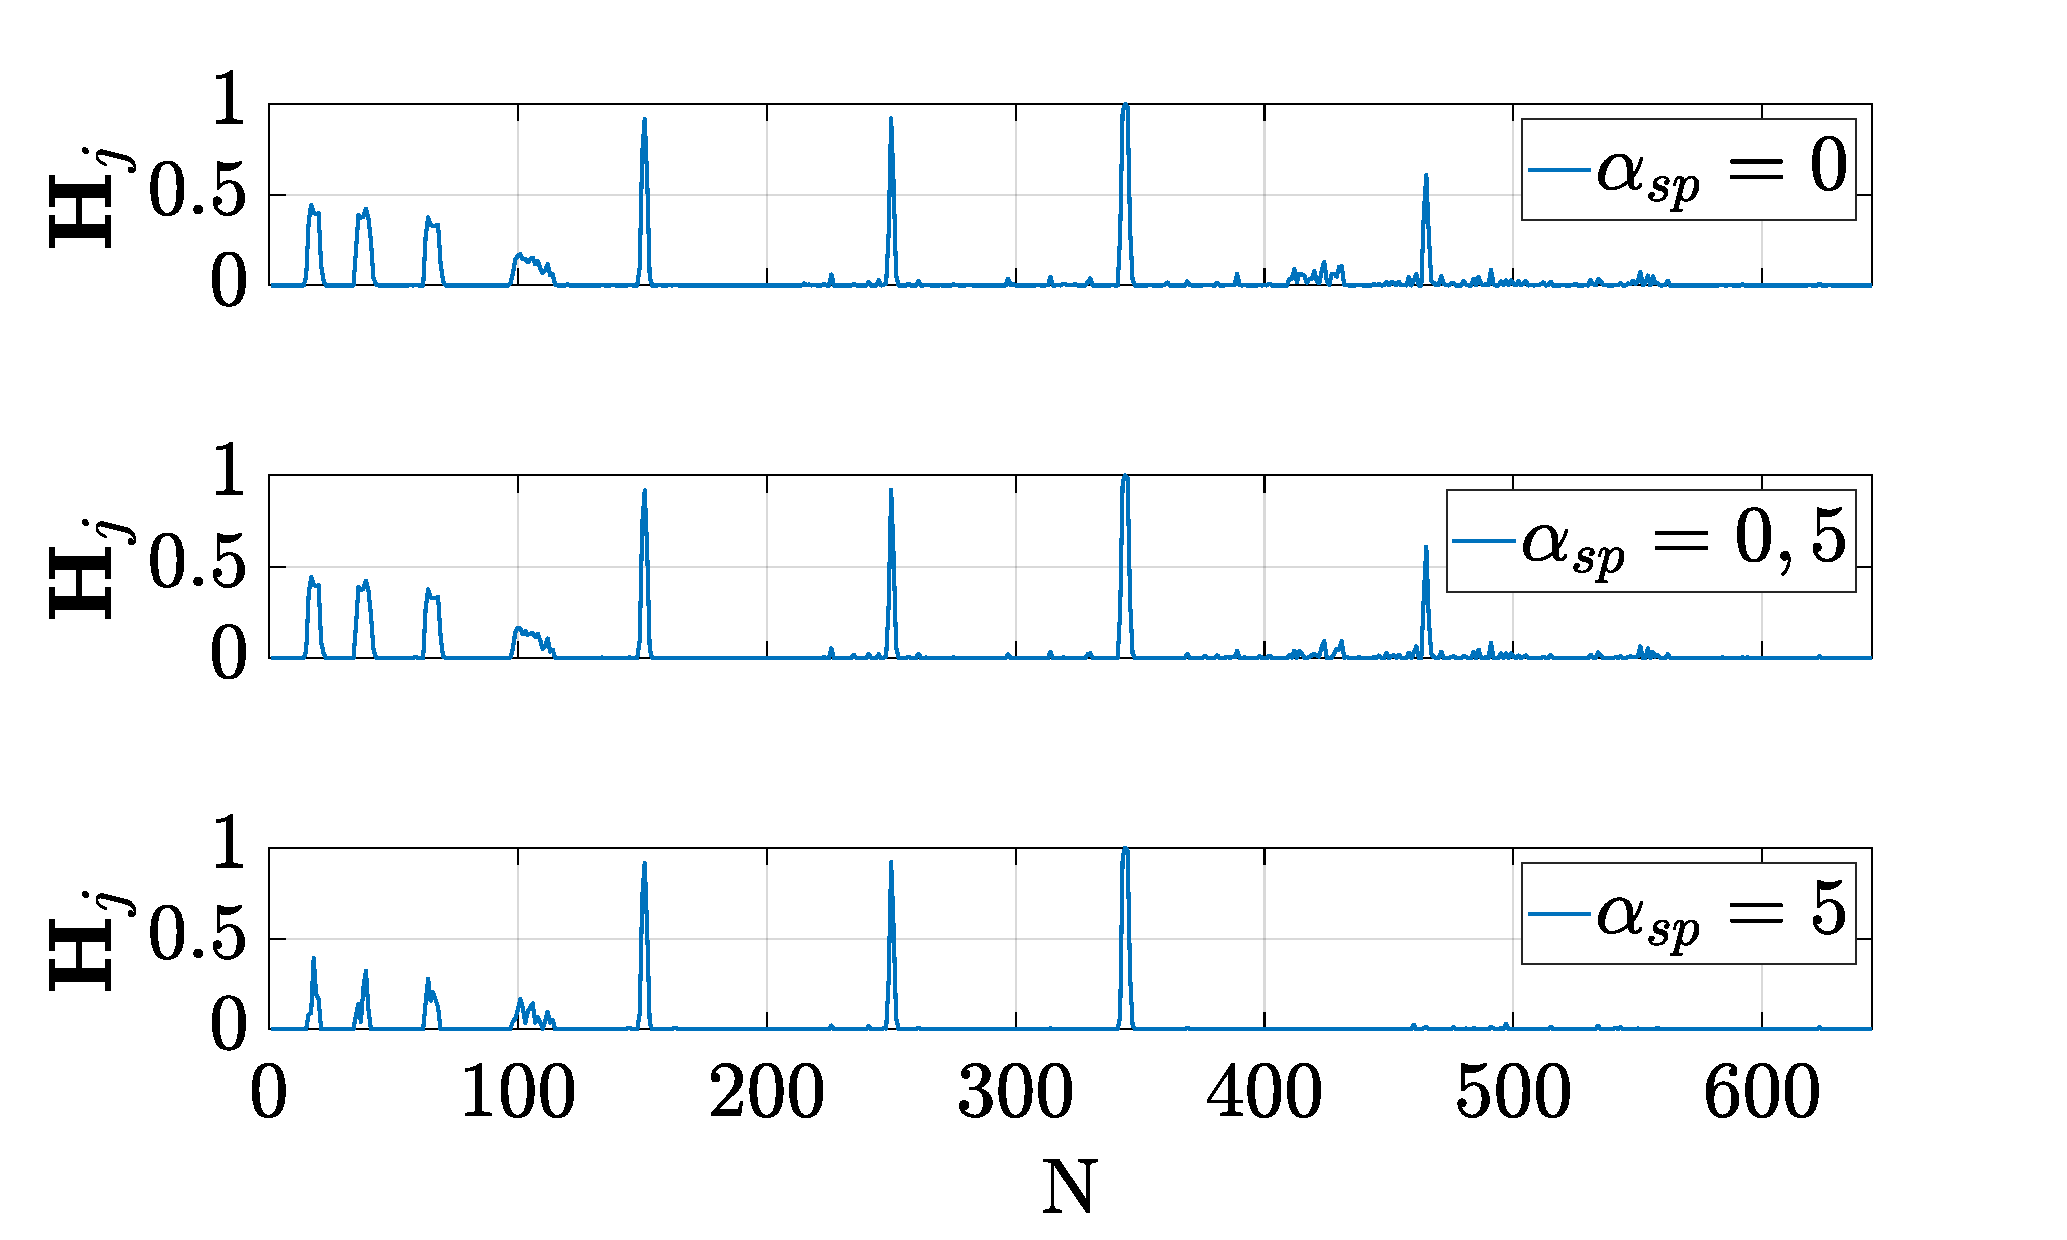
\includegraphics[width=.8\linewidth]{./figures/resultats/sparsity_example.pdf}
\caption{Exemple de l'effet de la parcimonie pour une scène du corpus \textit{alerte} pour $\alpha_{sp} \in \lbrace
0,~0,5,~5\rbrace$.}
\label{fig:sparsity_example}
\end{figure}


\subsection{Contrainte de régularité temporelle ou \textit{smooth} NMF}\label{part:smoothness}

La mise à jour de la matrice d'activation $\mathbf{H}$ se fait par défaut trame par trame sans considérer de liens entre les trames $n$ et les précédentes. Néanmoins, la plupart des sons réels ont une évolution temporelle lente. Prendre en compte l'évolution des trames temporelles adjacentes peut permettre que la forme des activateurs soit plus réaliste et que l'outil soit plus robuste dans la reconstruction du signal. Cette contrainte trouve son intérêt dans la musique (\cite{virtanen_sound_2003, fevotte_majorization-minimization_2011}) où les instruments (à l'exception des instruments percussifs) peuvent jouer des notes durant, au moins, plusieurs centaines de milli-secondes. Mais c'est aussi le cas au sein d'environnements sonores urbains où les sons (notamment le trafic routier) ont des variations lentes, de plusieurs secondes. L'une des approches les plus citées est celle de Virtanen \cite{virtanen_monaural_2007}, qui fut ensuite généralisée sous la forme d'un algorithme générique dans \cite{fevotte2017single}, avec l'ajout d'une contrainte $C_t(\mathbf{H})$ :

\begin{equation}\label{eq:smoothnessVirtanen}
C_t(\mathbf{H}) = \sum_{n=1}^K \sum_{n=2}^N \left(h_{kn} - h_{k(n-1)}\right)^2.
\end{equation}

La pondération de cette contrainte peut être constante sur tous les éléments ($\alpha_t$) ou bien être variable selon $k$ ($\alpha_{t,k})$ et doit donc être placée dans la somme. Par l'ajout de cette contrainte, les fortes variations d'un vecteur d'activation entre l'indice $n$ et $n-1$ sont pénalisées par la mise au \textit{carré} de leur distance. La mise à jour de $\mathbf{H}$ privilégie alors les variations plus lentes pour réduire le poids de la contrainte $C_t(\mathbf{H})$. L'algorithme de mise à jour devient :

\begin{equation}
\textbf{H}^{(i+1)} \leftarrow \textbf{H}^{(i)} \otimes\left(\frac{\textbf{W}^T \left[\left(\textbf{WH}^{(i)} \right)^{(\beta-2)} \otimes \textbf{V} \right] + 2 A \otimes \left(\overrightarrow{\mathbf{H}}^{(i)} + \overleftarrow{\mathbf{H}}^{(i)} \right)}{\textbf{W}^T \left[\textbf{WH}^{(i)} \right]^{(\beta-1)} + 2 A \otimes \left(\mathbf{H}^{(i)} + \overleftrightarrow{\mathbf{H}}^{(i)} \right)}\right)^{\gamma(\beta)}\label{eq:HupdateSmooth}
\end{equation}

avec

\begin{subequations}
\begin{align}
    A &=
\begin{bmatrix}
\alpha_{t,1} &  \cdots & \alpha_{t,1}  \\
\alpha_{t,2} & \dots & \alpha_{t,2}  \\
\vdots & \ddots &  \vdots \\
\alpha_{t,K} & \cdots & \alpha_{t,K}
\end{bmatrix}, \label{eq:subeq1}\\
    \overrightarrow{\mathbf{H}} &=
\begin{bmatrix}
0 & h_{1,1} & h_{1,2} & \cdots & h_{1,N-1}\\
0 & h_{2,1} & h_{2,2} & \cdots & h_{2,N-1}\\
\vdots & \vdots & \vdots & \ddots & \vdots\\
0 & h_{K,1} & h_{K,2} & \cdots & h_{K,N-1}\\
\end{bmatrix}, \label{eq:subeq2}\\
    \overleftarrow{\mathbf{H}} &=
\begin{bmatrix}
h_{1,2} & h_{1,3} & \cdots & h_{1,N} & 0\\
h_{2,2} & h_{2,3} & \cdots & h_{2,N} & 0\\
\vdots & \vdots & \ddots & \vdots & \vdots\\
h_{K,2} & h_{K,3} & \cdots & h_{K,N} & 0\\
\end{bmatrix}, \label{eq:subeq3}\\
    \overleftrightarrow{\mathbf{H}} &=
\begin{bmatrix}
0 & h_{1,2} & \cdots & h_{1,N-1} & 0\\
0 & h_{2,2} & \cdots & h_{2,N-1} & 0\\
\vdots & \vdots & \ddots & \vdots & \vdots\\
0 & h_{K,2} & \cdots & h_{K,N-1} & 0\\
\end{bmatrix}. \label{eq:subeq5}
\end{align}
\end{subequations}

$A$ résume les valeurs des contraintes selon $k$, $\overrightarrow{\mathbf{H}}$, les valeurs de $\mathbf{H}$ à l'instant $n-1$, $\overleftarrow{\mathbf{H}}$, les valeurs de $\mathbf{H}$ à l'instant $n+1$ et enfin $\overleftrightarrow{\mathbf{H}}$, les valeurs de $\mathbf{H}$ sur l'intervalle $\left[2,N-1 \right]$. L'impact du coefficient de pondération $\alpha_t$ sur les activations de $\mathbf{H}$ est représenté en Figure \ref{fig:smoothnessExample}. Plus cette pondération est forte plus l'allure des activateurs est régulière. C'est cet algorithme qui a été implémenté et testé pour les travaux de cette thèse.

\begin{figure}[hbtp]
\centering
	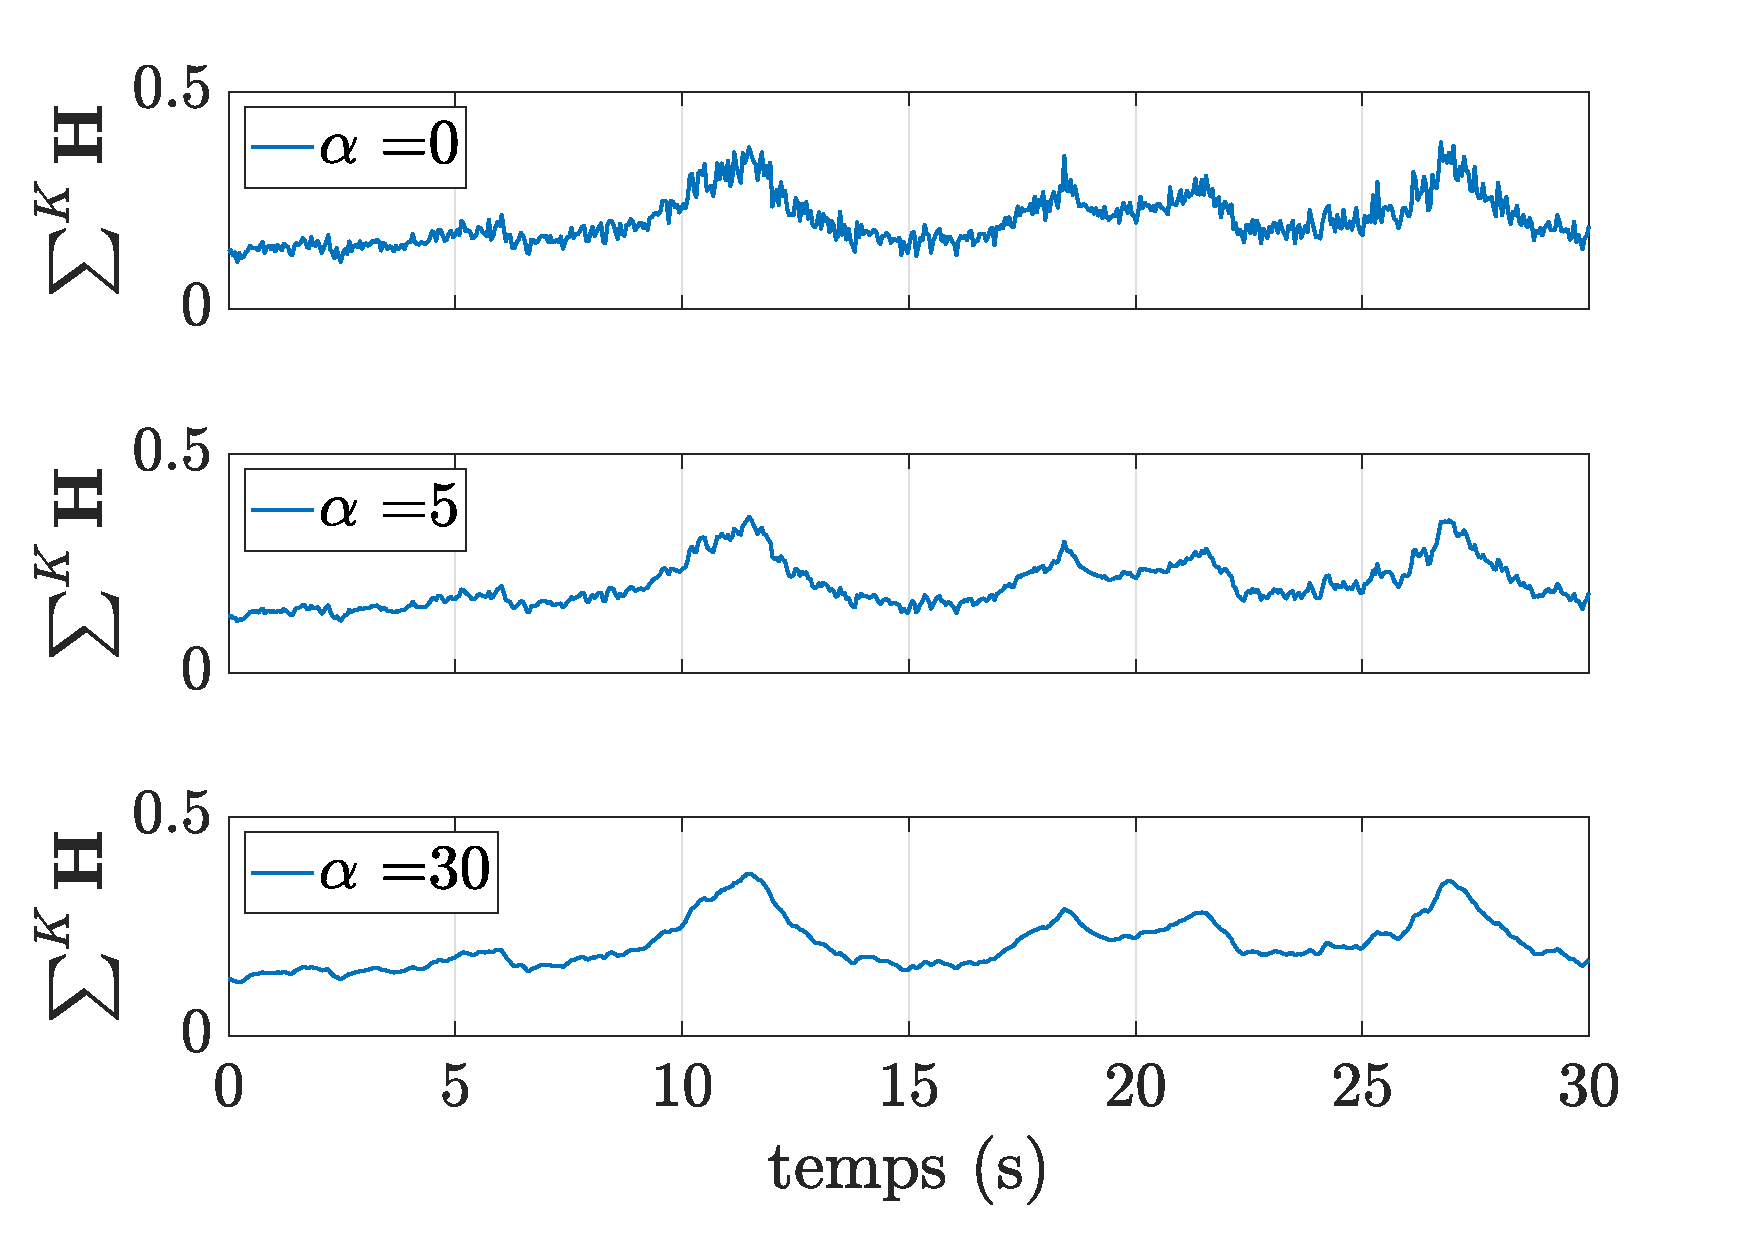
\includegraphics[width=0.7\linewidth]{./figures/NMF/smoothness_02.pdf}
\caption{Influence de la pondération $\alpha$ de la contrainte temporelle $C_t(\mathbf{H})$ sur la somme; selon $K$, des activateurs sur une scène audio de 30 secondes.}
\label{fig:smoothnessExample}
\end{figure}

D'autre approches ont également été étudiées. Dans, \cite{fevotte2011majorization}, dans le cas de la séparation de sources audio et la transcription d'un morceau de musique, une contrainte de régularité est proposée pour la divergence I-S. La particularité de la contrainte apposée est qu'elle se base elle-même sur la divergence I-S : $C_{I-S}(\mathbf{H}) = \sum_{k = 1}^{K} \sum_{n = 2}^{N}d_0(h_{k(n-1)} \vert h_{kn})$. L'algorithme de mise à jour est déduit à partir de l'algorithme de \textit{majorisation-minimisation} (voir partie \ref{part:majorisation-minimisation}). Dans \cite{essid2013smooth}, une contrainte, similaire à l'équation \ref{eq:smoothnessVirtanen} ($C_{MM}(\mathbf{H}) = \frac{1}{2}\sum_{k = 1}^{K} \sum_{n = 2}^{N}\left(h_{kn}-h_{k(n-1)}\right)^2$), est proposée dans le cas de la structuration de documents audiovisuels pour une divergence K-L avec, là encore, l'utilisation d'un algorithme de \textit{majorisation-minimisation}. Cette approche a été développée durant la thèse pour la divergence I-S et la distance EUC mais n'a pas été utilisée pour ces travaux. Les détails des calculs se situent en annexe \ref{annex:smoothNMF}.
Enfin on peut citer \cite{pascual2006nonsmooth} où une contrainte de \og non-smoothness \fg{} est considérée. L'idée est alors d'imposer de l'adoucissement dans la NMF sur une des deux matrices pour générer, en réaction inverse, de la parcimonie dans l'autre matrice. Le problème est ainsi posé :

\begin{equation}
\mathbf{V} \approx \mathbf{WSH}
\end{equation}

où $\mathbf{S}$ est une matrice de \textit{smoothness} telle que

\begin{equation}
\mathbf{S} = (1-\alpha_t)\mathbf{I}+\frac{\alpha}{K}\mathbf{11}^T
\end{equation}

avec $\mathbf{I}$ la matrice identité, $\mathbf{1}$ un vecteur unitaire et $\alpha_t$ un paramètre de \textit{smoothness} compris entre 0 et 1. Lorsque $\alpha = 0$, la régularité temporelle est nulle alors que pour $\alpha_t = 1$, le produit $\mathbf{SH}$ (ou $\mathbf{WS}$) génère un vecteur constant qui correspond à la moyenne des éléments de $\mathbf{H}$ (ou $\mathbf{W}$). Ce cas présente alors une parcimonie nulle puisque toute les entrées sont égales et non-nulles (là où une plus forte parcimonie présente des valeurs proches de 0).

\subsection{Autres contraintes}

D'autres contraintes existent dans la littérature mais ne seront pas étudiées dans ces travaux.
On peut citer une contrainte sur l'\textbf{harmonicité} des éléments de $\mathbf{W}$ qui a été proposée dans \cite{vincent2008harmonic} dans le cadre de la transcription d'une mélodie de piano. Le dictionnaire est alors décomposé en une somme de partiels sinusoïdes harmoniques ou inharmoniques pondérées selon une enveloppe spectrale. \cite{rigaud2012piano} propose une autre approche où une contrainte d'inharmonicité est imposée permettant à chaque élément de $\mathbf{W}$ de modifier la fréquence de chaque partiel tout en contraignant l'ensemble à suivre une loi d'inharmonicité.

La \textbf{NMF locale} a été proposée par \cite{li2001learning} qui contraint la fonction de coût avec trois pénalités : i) le nombre de bases $K$ doit être minimisé, ii) les bases doivent être le plus orthogonales que possible, iii) seules les bases qui donnent le plus d'informations sont conservées. Son application à la classification d'instruments de musique dans \cite{benetos2006musical} est toutefois peu efficace.

Dans le cadre de la NMF semi-supervisée, une contrainte est proposée dans \cite{yagi2012music}, puis étendue dans \cite{kitamura2014music} pour toute valeur de $\beta$, dans le cadre de la séparation de signaux musicaux afin de \textbf{maximiser la distance} (ou la divergence) entre le dictionnaire appris $\mathbf{W_s}$ et le dictionnaire libre $\mathbf{W_r}$ afin de s'assurer qu'un minimum d'information d'intérêt y soit intégré. Dans \cite{wang2016semi}, c'est une contrainte de propagation qui est considérée où un nouveau dictionnaire $\mathbf{W}$ est construit dans lequel les éléments similaires dans $\mathbf{W_r}$ à ceux appris et étiquetés sont pondérés. Dans \cite{lefevre2012semi}, la contrainte ajoutée consiste à pondérer le poids des éléments appris dans la reconstruction de $\mathbf{V}$ afin de donner une prépondérance différente des éléments non-appris.\\

\section{Conlusion du chapitre}

La Factorisation en Matrices Non-négative est une méthode qui permet l'approximation d'un spectrogramme en amplitude (ou en puissance) d'un enregistrement audio par le produit de deux matrices : $\mathbf{W}$, le dictionnaire composé de spectres sonores, et $\mathbf{H}$, la matrice d'activation. Différentes formes de NMF ont été proposées qui diffèrent selon les techniques d'apprentissage de leur dictionnaire (non-supervisée, supervisée et semi-supervisée) ou des contraintes qui y sont appliquées (parcimonie, régularité temporelle). Plusieurs de ces NMF sont implémentées dans le cas de ces travaux et testées en vue de déduire, sur des corpus de sons présentés dans le chapitre suivant, le niveau sonore du trafic routier.
La \textbf{NMF supervisée}, \textbf{semi-supervisée} et, celle proposée, \textbf{initialisée-seuillée} sont les trois approches retenues. L'influence de la contrainte de \textbf{régularité temporelle} $C_t(\mathbf{H})$  est  également observée pour un des corpus de sons dans le chapitre \ref{chap:grafic}. Les 3 $\beta$-divergences détaillées (\textbf{distance EUC} ($\beta = 2$), \textbf{divergence K-L} ($\beta = 1$) et \textbf{I-S} ($\beta = 0$)) seront celles utilisées sur chaque corpus.


%%%%%%%%%%%%%%%%%%%%%%%%%%%%%%%%%%%%%%%%%%%%%%%%%%%
%\bibliographystyle{unsrt}
%\bibliography{../bibliographie}
%
%\end{document}